% ---------------------------------------------------------------------------
% Author guideline and sample document for EG publication using LaTeX2e input
% D.Fellner, v1.13, Jul 31, 2008

\documentclass{egpubl}
\usepackage{eg2015}

% --- for  Annual CONFERENCE
%\ConferenceSubmission   % uncomment for Conference submission
\ConferencePaper        % uncomment for (final) Conference Paper
% \STAR                   % uncomment for STAR contribution
% \Tutorial               % uncomment for Tutorial contribution
% \ShortPresentation      % uncomment for (final) Short Conference Presentation
% \Areas                  % uncomment for Areas contribution
% \MedicalPrize           % uncomment for Medical Prize contribution
% \Education              % uncomment for Education contribution
%
% --- for  CGF Journal
% \JournalSubmission    % uncomment for submission to Computer Graphics Forum
% \JournalPaper         % uncomment for final version of Journal Paper
%
% --- for  CGF Journal: special issue
% \SpecialIssueSubmission    % uncomment for submission to Computer Graphics Forum, special issue
% \SpecialIssuePaper         % uncomment for final version of Journal Paper, special issue
%
% --- for  EG Workshop Proceedings
% \WsSubmission    % uncomment for submission to EG Workshop
% \WsPaper         % uncomment for final version of EG Workshop contribution
%
 \electronicVersion % can be used both for the printed and electronic version

% !! *please* don't change anything above
% !! unless you REALLY know what you are doing
% ------------------------------------------------------------------------

% for including postscript figures
% mind: package option 'draft' will replace PS figure by a filname within a frame
%\ifpdf \usepackage[pdftex]{graphicx} \pdfcompresslevel=9
%\else \usepackage[dvips]{graphicx} \fi

\PrintedOrElectronic

% prepare for electronic version of your document
\usepackage{t1enc,dfadobe}

\usepackage{egweblnk}
\usepackage{cite}
\usepackage{balance}

% For backwards compatibility to old LaTeX type font selection.
% Uncomment if your document adheres to LaTeX2e recommendations.
% \let\rm=\rmfamily    \let\sf=\sffamily    \let\tt=\ttfamily
% \let\it=\itshape     \let\sl=\slshape     \let\sc=\scshape
% \let\bf=\bfseries

% end of prologue

%\input{EGauthorGuidelines-body.inc}
% ---------------------------------------------------------------------
% EG author guidelines plus sample file for EG publication using LaTeX2e input
% D.Fellner, v1.17, Sep 23, 2010


\title[GVD of Closely-Spaced Objects]%
      {\red{Approximating} the Generalized Voronoi Diagram of Closely Spaced Objects}

% for anonymous conference submission please enter your SUBMISSION ID
% instead of the author's name (and leave the affiliation blank) !!
% For Computer Graphics Forum: Please use the abbreviation of your first name.

%% author example
%\author[D. Fellner \& S. Behnke]
%       {D.\,W. Fellner\thanks{Chairman Eurographics Publications Board}$^{1,2}$
%        and S. Behnke$^{2}$
%        S. Spencer$^2$\thanks{Chairman Siggraph Publications Board} \\
%         $^1$TU Darmstadt \& Fraunhofer IGD, Germany \\
%         $^2$Institut f{\"u}r ComputerGraphik \& Wissensvisualisierung, TU Graz, Austria
%       }

\author[J. Edwards \& E. Daniel \& V. Pascucci \& C. Bajaj]
%       {John Edwards\thanks{jedwards@sci.utah.edu}$^1$ and
       {John Edwards$^1$ and
         Eric Daniel$^2$ and
         Valerio Pascucci$^1$ and
         Chandrajit Bajaj$^3$ \\
%         $^1$Scientific Computing and Imaging Institute, University of Utah \\
%         $^2$Google, Inc. \\
%         \footnotesize{$^3$The University of Texas at Austin}
         \parbox[t]{10cm}{\centering $^1$Scientific Computing and Imaging Institute, University of Utah \\
         $^2$Google, Inc. \\
         \footnotesize{$^3$The University of Texas at Austin}}
       }
%\author[paper1040]
%       {paper1040}

% ------------------------------------------------------------------------

% if the Editors-in-Chief have given you the data, you may uncomment
% the following five lines and insert it here
%
% \volume{27}   % the volume in which the issue will be published;
% \issue{1}     % the issue number of the publication
% \pStartPage{1}      % set starting page

\renewcommand{\paragraph}[1]{\noindent \textbf{#1}}
%\usepackage{amsmath,amsthm,amsfonts,amscd,amssymb,amstext} 
\usepackage{amsmath,amsfonts,amscd,amssymb,amstext} 
\usepackage{mathrsfs}
				% Some packages to write mathematics.
\usepackage{overpic}
\usepackage{eucal} 	 	% Euler fonts
\usepackage{verbatim}      	% Allows quoting source with commands.
\usepackage{makeidx}       	% Package to make an index.
%\usepackage{citesort}         	% 
\usepackage{subfig}
\usepackage{graphicx}
\usepackage{url}		% Allows good typesetting of web URLs.
\usepackage{multirow}
%\usepackage[linesnumbered, noline]{algorithm2e}
%\usepackage[boxed, noline]{algorithm2e}
\usepackage[ruled]{algorithm2e}
\usepackage{booktabs}
\usepackage{tabularx}
\usepackage{array}
\usepackage{color}
\usepackage{tikz}
% To balance the columns at the end
\usepackage{balance}
\usepackage[mediumspace,mediumqspace,Grey,squaren]{SIunits}
%\usepackage{draftcopy}		% Uncomment this line to have the
				% word, "DRAFT," as a background
				% "watermark" on all of the pages of
				% of your draft versions. When ready
				% to generate your final copy, re-comment
				% it out with a percent sign to remove
				% the word draft before you re-run
				% Makediss for the last time.
\usepackage[normalem]{ulem}

\definecolor{bostonuniversityred}{rgb}{0.8, 0.0, 0.0}

%------------------------------------------------------------
% Custom commands
%------------------------------------------------------------
%\newcommand{\old}[1]{\textcolor{blue}{\sout{#1}}}
\newcommand{\old}[1]{}

%\newcommand{\red}[1]{\textcolor{red}{#1}}
%\newcommand{\red}[1]{\textcolor{bostonuniversityred}{#1}}
\newcommand{\red}[1]{#1}

%\newcommand{\reconstruct}{RECONSTRUCT\textsuperscript{\texttrademark}}
%\newcommand{\tm}{\textsuperscript{\texttrademark}}
\newcommand{\tm}{$^1$}
\newcommand{\addref}{\red{REF}}
\newcommand{\mathtext}[1]{\text{#1}}
\newcommand{\etal}{et al.\ }
\newcommand{\algorithmspace}{\vspace{8pt}}
\newcommand{\glfs}{\emph{glfs}}

\renewcommand{\vec}[1]{\mathbf{#1}}

\newcommand{\centercell}[1]{\multicolumn{1}{c}{#1}}
\newcolumntype{x}[1]{>{\centering\arraybackslash\hspace{0pt}}m{#1}}
\newcolumntype{y}[1]{>{\centering\arraybackslash\hspace{0pt}}m{#1\textwidth}}
\newcolumntype{M}{>{\centering\arraybackslash}m{1cm}}

\DeclareMathOperator*{\argmin}{arg\,min}
\DeclareMathOperator*{\argmax}{arg\,max}

\newcommand{\BigO}[1]{\ensuremath{\operatorname{O}\left(#1\right)}}
\newcommand{\centroid}{\mathscr{C}}
\newcommand{\iring}{\mathscr{R}}

% aligned
\renewcommand{\d}{\delta}
\newcommand{\vempty}{\mathscr{E}}
\newcommand{\e}{\epsilon}
\newcommand{\dist}{\mathtext{dist}}
\newcommand{\ball}{\mathscr{B}}


\newcommand{\hgt}{22mm}

%--------------------------------------------------
% Theorem environments (amsthm package required)
%--------------------------------------------------
% \theoremstyle{plain} %% This is the default
\newtheorem{theorem}{Theorem}
\newtheorem{lemma}{Lemma}
\newtheorem{corollary}{Corollary}
\newtheorem{conjecture}{Conjecture}
\newtheorem{crit}{Criterion}
\newtheorem{condition}{Condition}
\newtheorem{fact}{Fact}

%\theoremstyle{definition}
%\newtheorem{defn}{Definition}[section]

%\theoremstyle{remark}
%\newtheorem{rem}{Remark}[section]
%\newtheorem*{notation}{Notation}

%\numberwithin{equation}{section}

%--------------------------------------------------
% Tight enumerations
%--------------------------------------------------
\newenvironment{tightenumerate}{
\begin{enumerate}
  \setlength{\itemsep}{1pt}
  \setlength{\parskip}{0pt}
  \setlength{\parsep}{0pt}
}{\end{enumerate}
}
\newenvironment{tightitemize}{
\begin{itemize}
  \setlength{\itemsep}{1pt}
  \setlength{\parskip}{0pt}
  \setlength{\parsep}{0pt}
}{\end{itemize}
}

%--------------------------------------------------
% Add figs to graphics path
%--------------------------------------------------
\graphicspath{{./}{./figs/}}

\newcolumntype{H}{@{}>{\lrbox0}l<{\endlrbox}}


%-------------------------------------------------------------------------
\begin{document}

%\teaser{
%  \subfloat[][]{
%    \label{fig:gears1}
%    \begin{tikzpicture}
%      \node[anchor=south west,inner sep=0] at (0,0) {
%        \begin{tabular}[b]{c}
%          \includegraphics[height=0.8in]{gears-far1.png} \\
%          \includegraphics[height=0.8in]{gears-close1.png}
%        \end{tabular}
%      };
%      \draw[black,thick] (1.4,3.2) rectangle (2.0,3.6);
%      \draw[black,dashed] (1.4,3.6) -- (0.22,2.15);
%      \draw[black,dashed] (2.0,3.6) -- (2.95,2.15);
%      \draw[black,thick] (0.22,0.1) rectangle (2.95,2.15);
%    \end{tikzpicture}
%  }
%  \subfloat[][]{
%    \label{fig:gears}
%    \begin{tikzpicture}
%      \node[anchor=south west,inner sep=0] at (0,0) {
%        \begin{tabular}[b]{c}
%          \includegraphics[height=0.8in]{gears-far4.png} \\
%          \includegraphics[height=0.8in]{gears-close4.png}
%        \end{tabular}
%      };
%      \draw[black,thick] (1.3,3.1) rectangle (1.9,3.5);
%      \draw[black,dashed] (1.3,3.5) -- (0.22,2.15);
%      \draw[black,dashed] (1.9,3.5) -- (2.92,2.15);
%      \draw[black,thick] (0.22,0.1) rectangle (2.92,2.15);
%    \end{tikzpicture}
%  }
%  \hspace{3mm}
%  \subfloat[][]{
%    \label{fig:knife}
%    \includegraphics[trim=4cm 0cm 4cm 2.5cm, clip=true, height=1.4in]
%                    {knife-above/slice-00000.png}
%  }
%  \subfloat[][]{
%    \label{fig:knife2}
%    \includegraphics[trim=2mm 0cm 2mm 2cm, clip=true, height=1.4in]
%                    {knife-above/slice-00110.png}
%  }
%  \caption{Two example applications of the \red{approximated} generalized Voronoi diagram (GVD) computed by our novel, adaptive algorithm. Previous GVD methods require a gridded space of $2^{24}$ (gears dataset) and $2^{36}$ (knives dataset) voxels to resolve the closely spaced objects.
%    \protect\subref{fig:gears1} Two gears with regions of very tight spacing.
%    \protect\subref{fig:gears} The GVD of the gears model.  The surface is colored red in areas of very close tolerance.
%    \protect\subref{fig:knife} Three butter knives in a wood block.  To animate removal of the knives without intersecting the block requires extreme care because of close mesh spacing.
%    \protect\subref{fig:knife2} Intersection-free motion is guaranteed by computing motion vectors based on the GVD and allowing motion only within a Voronoi cell.
%  }
%  \label{fig:teaser}
%}

\maketitle

\begin{abstract}
We present an algorithm to compute \red{an approximation of} the generalized Voronoi diagram (GVD) on arbitrary collections of 2D or 3D geometric objects.  In particular, we focus on datasets with closely spaced objects; GVD approximation is expensive and sometimes intractable on these datasets using previous algorithms.  With our approach, the GVD can be computed using commodity hardware even on datasets with many, extremely tightly packed objects.  Our approach is to subdivide the space with an octree that is represented with an adjacency structure. We then use a novel adaptive distance transform to compute the distance function on octree vertices. The computed distance field is sampled more densely in areas of close object spacing, enabling robust and parallelizable GVD surface generation.  We demonstrate our method on a variety of data and show example applications of the GVD in 2D and 3D. \\

%   Leave one blank line after the abstract, 
%   then add the subject categories according to the ACM Classification Index 
%   (see http://www.acm.org/class/1998/).

\begin{classification} % according to http://www.acm.org/class/1998/
  \CCScat{I.3.5}{Computer Graphics}{Computational Geometry and Object Modeling}{Boundary representations}
  \CCScat{I.3.6}{Computer Graphics}{Methodology and Techniques}{Graphics data structures and data types}
  %\CCScat{Computer Graphics}{I.3.3}{Picture/Image Generation}{Line and curve generation}
\end{classification}

\end{abstract}

%-------------------------------------------------------------------------
% Body
%-------------------------------------------------------------------------

%-------------------------------------------------------------------------------
% introduction
%-------------------------------------------------------------------------------
\section{Introduction}
\label{sec:intro}
%An unsigned distance function $f:\mathbb{R}^n\to\mathbb{R}$ gives the minimum distance from a point $p$ to an object $S$ modulus some error, that is, $\inf_{q \in S}{\dist(p, q)} + \epsilon(p)$ where $\dist(p, q)$ is the distance between points $p$ and $q$ and $\epsilon(p)$ is an error measure. Unsigned distance functions, and especially their cousin, the signed distance function, which endows the distance with a sign depending on whether $p$ is inside or outside of an object, are applicable in a large number of applications, including motion path planning, geospatial distance queries, object representation and processing, image quantization, and level-set functions.  One important construct that can be derived from a distance function is the generalized Voronoi diagram (GVD), a generalization of the Voronoi diagram for point sets.
%
%Given a set of seed points $\{x_i\}$, or sites, the Voronoi diagram (VD) is the locus of points with at least two closest sites.  It divides space into cells $\{VC_i\}$ such that every point in a cell $VC_i$ is closer to $x_i$ than to any other site.  That is, given a space $X$ where the distance between two points $a,b \in X$ is given as $\dist(a, b)$, the Voronoi cell for a site $x_i$ is $VC_i = \{p \in X| \dist(p, x_i) < \dist(p, x_j), j \ne i\}$. If site $x_i$ is given the label $i$ then we say that every point $p \in VC_i$ has label $i$.  The VD is a bisector of the space between sites and is piecewise linear.
%
%The generalized Voronoi diagram lifts the restriction that sites be points, allowing arbitrary objects to be sites.  The definition of the GVD is the same as that of the VD: given a set of objects $\{S_i\}$, a generalized Voronoi cell (GVC) is defined as GVC$_i = \{p \in X | \dist(p, S_i) < \dist(p, S_j), j \ne i\}$ where $\dist(p, S_i) = \inf_{q \in S_i}{\dist(p, q)}$ and can be approximated by a distance function.  Because sites can be arbitrary objects, the GVD is higher order in general \cite{boissonnat2006curved}.  For example, the bisector of a point and a line is a quadratic curve.  Generalized Voronoi diagrams are difficult to compute analytically in general \cite{boissonnat2006curved,hoff1999fast} and so most approaches use a distance field computed by a distance function to construct an approximate GVD.
%
%In order for the distance function to be useful in building a GVD it must not only yield a distance, but also the label of the closest site, that is, $f:\mathbb{R}^n\to\mathbb{R}\times L$ where $L$ is the set of all labels.  The GVD is then exactly the set of critical points at which the label changes. We note that the medial axis is the analog to the bisector in a continuous setting, that is, when an infinite number of point sites are used.
%
%Distance transforms (DTs) are a popular method of computing a distance field and include chamfer DTs, vector DTs, and the fast marching method \cite{jones20063d}. The majority of existing distance transforms compute distances over a grid.  While appropriate for many applications, uniform grids require a prohibitively large number of pixels (voxels) when the spatial extent is large compared to spacing between objects.  Adaptive distance fields (ADFs) \cite{strain1999fast,frisken2000adaptively} use spatial subdivision methods, such as quadtrees and octrees, to compute distances at higher resolution in areas of detailed object features.

The generalized Voronoi diagram (GVD) is an important structure that divides space into a complex of generalized Voronoi cells (GVCs) around objects.  Similar to the ordinary Voronoi diagram, each GVC contains exactly one object, or site, and every point in the GVC is closer to its contained object than to any other object.  The generalized Voronoi diagram is the boundary of the cell complex, and thus every point on the GVD is equidistant from two or more closest objects.  Applications of the GVD range from motion path planning to GIS analysis to mosaicking.

Ordinary Voronoi diagrams have been studied extensively and efficient algorithms exist to compute them, but the GVD is difficult to compute analytically in general \cite{boissonnat2006curved,hoff1999fast} and so the majority of approaches compute an approximation.  Whereas most algorithms are efficient and robust on certain datasets, all algorithms to our knowledge require inordinate amounts of memory on datasets where objects are very closely spaced relative to the size of the domain.  The failures occur because the space is uniformly gridded.  In such approaches, voxel size must be small enough to resolve object spacings, and if two objects are very close to each other the number of voxels can become prohibitively large.

We present an algorithm to compute a GVD approximation on arbitrary datasets, including those with closely spaced objects.  The approach applies a distance transform over an octree representation of the objects.  Our octree, its associated data structure, and our distance transform are novel and optimized to GVD \red{approximation. For the remainder of the paper, ``GVD'' will refer to the approximated Generalized Voronoi Diagram.}

This paper demonstrates GVD computation on data beyond the computational abilities of previous algorithms, unlocking interesting and important applications.  Our approach allows GVD-based proximity queries and other applications using a larger class of meaningful datasets.


%\paragraph{Main contributions} In computation of a GVD, we are less concerned with details of objects; rather, we adapt subdivision to most efficiently compute a distance field for GVD computation.  Our main contributions are fourfold.\footnote{Our algorithms support both 2D and 3D. For simplicity, we will use 3D terms (e.g. octree rather than quadtree) when discussing dimension-independent concepts, but will revert to 2D terms when convenient.}

\paragraph{Main contributions} The three primary technical contributions described in the paper are as follows.
%This paper describes three technical contributions relating to GVD computation.

\begin{enumerate}
\item Most octree decompositions of objects resolve for object feature retention, but ours resolves only for object-object separation, which makes our subdivision computation largely independent of object complexity.  Further, our octree data structure optimizes for octree vertex neighbor finding
%gains memory savings
by storing cell vertices in an adjacency list rather than storing cells hierarchically.
%, and by omitting spatial information from the data structure.
\item Our distance transform is computed after the octree is built and uses a scheme that requires $\BigO{N\log{N}+M}$ distance computations where $N$ is the number of octree leaf cells and $M$ is a measure of object complexity (e.g., number of polyhedron facets).  Distances are computed on octree vertices with a conjectured error bound.%and are error bounded.
\item We trace out the GVD over the octree distance field using an efficient and parallelizable $\BigO{N}$ algorithm.  The GVD is guaranteed to separate each object into its own generalized Voronoi cell, i.e., any path from a point $p$ on object $S_i$ to a point $q$ on object $S_j$ must intersect the GVD, a guarantee that is not usually made by uniformly gridded methods.
%\item We present an adaptive subdivision scheme that subdivides as necessary to resolve objects.  Object features are resolved only if they closely approach another object.  Our octree data structure gains memory savings by storing cell vertices in an adjacency list rather than storing cells hierarchically, and by omitting spatial information from the data structure.
%\item Our distance transform is computed after the octree is built and uses a scheme that requires $\BigO{N+M}$ distance computations where $N$ is the number of octree leaf cells and $M$ is a measure of object complexity (e.g. number of facets for polyhedra or local feature size for curved surfaces).  Distances are computed on octree vertices and are error bounded.
%\item We trace out the GVD over the octree distance field using an efficient $\BigO{N}$ algorithm.  The GVD is guaranteed to separate each object into its own generalized Voronoi cell, i.e., any path from a point $p \in S_i$ to a point $q \in S_j$ must intersect the GVD, a guarantee that is not usually made by uniformly gridded methods.
%\item We demonstrate various applications of the GVD in 2 and 3 dimensions, including motion path planning, pruning of occluding structures, and exploded diagrams.
\end{enumerate}

We demonstrate various applications of the GVD in two and three dimensions, including motion path planning, proximity queries, and exploded diagrams.

%Our algorithm has two primary products, a sampled distance field and a GVD.  As the GVD is our primary motivation, the distance transform is designed to support efficient GVD computation.  We have four main steps in our algorithm: 1) build the octree over the set of objects; 2) compute distances on octree vertices using a wavefront expansion; 3) resolve ambiguous cells through further subdivision; 4) compute the GVD surface by finding octree edges with differing end labels.  We discuss each step in detail.

Our GVD algorithm has four main steps: 1) build the octree over the set of objects; 2) compute distances on octree vertices using a wavefront expansion; 3) resolve ambiguous cells through further subdivision; and 4) compute the GVD surface by finding octree edges with differing end labels.  After a discussion of related work, we discuss each step in detail and present applications.

%-------------------------------------------------------------------------------
% Related work
%-------------------------------------------------------------------------------
\section{Related work}
Related work falls into two categories: algorithms that compute the GVD and algorithms that compute distance fields, many of which are adaptive.

%\paragraph{To review}
%\begin{tightenumerate}
%\item \red{\cite{karras2012maximizing} - GPU octree. Fast, parallel construction of octree of points. Morton codes, so limited to depth 10 when using 32-bit integers.  Since we use n points, we know that number of leaf nodes <= n, so we can block-allocate the octree.  We can't do this in our case.}
%%\item \cite{decoro2007realtime} - GPU ``probabilistic octree'' - not really applicable
%\item \red{\cite{bedorf2012sparse} - GPU octree. Points only.  Morton codes.}
%\item \red{\cite{laine2011efficient} - GPU octree.  Builds over triangles, so not just points.  Octree size not known a priori.  Designed for rendering.  Speed of octree generation is similar (on the order of one second per Mb of octree), but apples-to-apples compare is not possible.}
%\item \red{\cite{baert2013out} - GPU octree, out-of-core.  Resolution must be determined a priori for partitioning of triangle mesh.  We don't know what resolution we'll need.  Designed for speed of construction, but is still reasonably close to ours (roughly 0.5 seconds per Mb of octree)}
%\item \red{\cite{zhou2011data} - GPU octree.  Points only.  Morton codes, so limited to depth 10 when using 32-bit integers.}
%\item \red{\cite{sud2006fast} - Collision detection. GPU: Uniform grid, error in distance field is bounded, but error is proportional to grid cell size.  Used in collision detection, so error upper bound is used to detect in N-body problem and then better techniques are used if GVD-based test is positive.}
%\item \red{\cite{fischer2006fast} - VD. GPU: k-order VD with point sites}
%\item \red{\cite{hsieh2005simple} - GVD. GPU: voronoi sites restricted to points, lines and triangles, uniform}
%\item \red{\cite{vleugels1998approximating} - GVD. adaptive, but sites are convex. no parallelism, expensive.}
%\item \cite{sud2008real} - Path planning. GPU-based path planning of multiple agents.  Uniform.  \ref{Idea: try computing shortest path in 2D example using ``uniform grid'' or lower-resolution octree}
%\item Gigavoxels and PantaRay (pointed out by reviewer 97), along with other out-of-core LOD rendering and lighting approaches, typically stream to GPU memory only the data necessary for rendering, which could potentially be useful for large-scale datasets that require out-of-core GVD computation.
%\end{tightenumerate}

\paragraph{Generalized Voronoi diagrams}
A theoretical framework for generalized Voronoi diagrams can be found in Boissonnat \etal \shortcite{boissonnat2006curved}. Ordinary Voronoi diagrams are well studied and efficient algorithms exist that compute them exactly \cite{de2008computational}, but exact algorithms for the generalized Voronoi diagram are limited to a small set of special cases \cite{lee1982medial,karavelas2004robust}. In an early work, Lavender \etal \shortcite{lavender1992voronoi} define and compute GVDs over a set of solid models using an octree.  Etzion and Rappoport \shortcite{etzion2002computing} represent the GVD bisector symbolically for lazy evaluation, but are limited to sites that are polyhedra.  Boada \etal \shortcite{boada2002voronoi,boada2008approximations} use an adaptive approach to GVD computation, but their algorithm is restricted to GVDs with connected regions and is inefficient for polyhedral objects with many facets.  Two other works are adaptive \cite{teichmann1997polygonal,vleugels1998approximating} but are computationally expensive and are restricted to convex sites.
%Teichmann and Teller \shortcite{teichmann1997polygonal} compute the GVD by adaptively subdividing space into a tetrahedral complex, but the method is memory and computationally expensive and is restricted to objects composed of triangles.  The method of Vleugels and Overmars \shortcite{vleugels1998approximating} is also adaptive but sites must be convex. no parallelism, expensive.

In recent years Voronoi diagram algorithms that take advantage of fast graphics hardware have become more common \cite{cao2010parallel,fischer2006fast,hsieh2005simple,rong2007variants,sud2006interactive,sud2006fast,hoff1999fast,wu2008gpu}.  These algorithms are efficient and generalize well to the GVD, but most are limited to a subset of site types.  More importantly, all of them use uniform grids and require an extraordinary number of voxels to resolve closely spaced objects (for example, Figs. \ref{fig:knife} and \ref{fig:path} would require $2^{36}$ and $2^{48}$ voxels, respectively).  To our knowledge, ours is the first fully adaptive algorithm that computes the generalized Voronoi diagram for arbitrary datasets.  %We know of no fully adaptive algorithm that computes the generalized Voronoi diagram on arbitrary datasets.

\paragraph{Distance fields and octrees}
The GVD is a subset of the locus of distance field critical points, a property that we take advantage of. In that light, the GVD could be a post-processing step to any method that computes a distance field.  Distance transforms compute a distance field, but most are uniformly gridded \cite{jones20063d} and are thus no more suitable than GVD algorithms that use the GPU.
%Most sequential distance transforms, including chamfer distance transforms, vector distance transforms and the fast marching method \cite{jones20063d}, lack adaptivity and thus require large amounts of memory when feature size is small compared to bounding box size.  However, there has been some excellent work in adaptive methods, mostly in the context of building a distance field for a single object.

% JME: note that in the Bastos work, ``reconstruction'' is reconstruction
% of the surface from the octree at rendering time.
Two seminal works adaptively compute the Adaptive Distance Field (ADF) on octree vertices.  Strain~\shortcite{strain1999fast} fully resolves the octree everywhere on the object surface, and Frisken \etal~\shortcite{frisken2000adaptively} resolve the octree fully only in areas of small local feature size.  Both approaches are designed to retain features of a single object rather than resolving between multiple objects, as is required for GVD computation.  Qu \etal \shortcite{qu2004feature} implement an energy-minimizing distance field algorithm that preserves features at the expense of efficiency.  Many recent works on fast octree construction using the GPU are limited to point sites \cite{bedorf2012sparse,karras2012maximizing,zhou2011data}. Most octree approaches that support surfaces \cite{baert2013out,crassin2009gigavoxels,laine2011efficient,lefebvre2007compressed} are designed for efficient rendering, and actual construction of the octree is implemented on the CPU.
%These algorithms require a specified maximum resolution \textit{a priori}, but in our case, maximum resolution is determined by minimum object spacing, which is computed during octree construction.

Two works \cite{bastos2008gpu,park2010cuda} implement the ADF using GPU parallelism to compute the distance value at sample points, but building the octree itself is done sequentially.  Yin \etal~\shortcite{yin2011fast} compute the distance field entirely on the GPU using a bottom-up approach by initially subdividing into a complete octree, resulting in memory usage that is no better than using a uniform grid.  A method by Kim and Liu~\shortcite{kim2014exact} computes the octree and a BVH entirely on the GPU. However, octree construction is performed on barycenters of triangles, and so a leaf octree cell can have an arbitrary number of triangle intersections as long as it contains no more than one triangle's barycenter.  We have found no GPU octree construction method that can resolve between objects.

%Two works \cite{bastos2008gpu,yin2011fast} have implemented Adaptive Distance Fields using GPGPU.  Bastos and Celes \shortcite{bastos2008gpu} focus on data structures that are efficient for rendering, and their octree construction times appear to be an order of magnitude slower than ours (exact timings were not reported).  Yin \etal \shortcite{yin2011fast} use a bottom-up approach, initially subdividing into a complete octree, yielding a uniform grid at every octree level.  Thus, the memory usage is no better than using a uniform grid.

%Strain~\shortcite{strain1999fast} computes the distance field exactly at vertices of an octree for redistancing when computing level sets.  The octree is fully resolved everywhere on the object surface.  Frisken \etal~\shortcite{frisken2000adaptively} proposed a similar approach that resolves the octree fully only in areas of small local feature size. Storage of the octree was later improved by Lefebvre and Hoppe \shortcite{lefebvre2007compressed} who introduced a compression scheme while maintaining fast random spatial access, which unfortunately requires high compression times.  Qu \etal \shortcite{qu2004feature} implement a distance-field algorithm that preserves features at the expense of efficiency.  Two works \cite{bastos2008gpu,yin2011fast} have implemented Adaptive Distance Fields using GPGPU.  Bastos and Celes \shortcite{bastos2008gpu} focus on data structures that are efficient for rendering, and their ADF construction times appear to be an order of magnitude slower than ours (unfortunately they don't report exact timings).  Yin \etal \shortcite{yin2011fast} use a bottom-up approach, initially subdividing into a complete octree, yielding a uniform grid at every octree level.  Thus, the memory usage is even higher than using a uniform grid, making it impossible to resolve very closely spaced objects on commodity hardware.

%\paragraph{Octrees}
%Our approach computes a distance field over octree vertices. Octree construction is a major and expensive step, and a large amount of recent research has focused on GPU octree construction.  The fastest approaches are limited to point sites \cite{bedorf2012sparse,karras2012maximizing,zhou2011data}. Approaches that support surfaces \cite{crassin2009gigavoxels,laine2011efficient,lefebvre2007compressed} are generally designed for fast access in rendering applications and have slow octree construction times.
%Our approach computes a distance field over octree vertices. Octree construction is a major step in our pipeline. Recent works on fast octree construction using the GPU are limited to point sites \cite{bedorf2012sparse,karras2012maximizing,zhou2011data}. Most octree approaches that support surfaces \cite{baert2013out,crassin2009gigavoxels,laine2011efficient,lefebvre2007compressed} are designed for efficient rendering, and actual construction of the octree is implemented on the CPU.  These algorithms require a specified maximum resolution \textit{a priori}; this is a reasonable request for rendering applications, but in our case, maximum resolution is determined by minimum object spacing, which is computed \textit{during} octree construction.

%A non-GPU approach of note is that of Baert \etal~\shortcite{baert2013out}, which generates an octree on out-of-core data.  Their algorithm requires a specified maximum resolution \textit{a priori}; this is a reasonable request for rendering applications, where the user can dictate a desired resolution, but in our case, maximum resolution is determined by minimum object spacing, which can be computed only \textit{after} octree construction.

%Park \etal~\shortcite{park2010cuda} implement a distance field using massive GPU parallelism to compute the signed distance value for a sample point, but building the octree itself is done sequentially.  An improved method by Kim and Liu~\shortcite{kim2014exact} computes the octree and a BVH entirely on the GPU. However, octree construction is performed on barycenters of triangles, and so an octree cell can have an arbitrary number of triangle intersections, but it will be subdivided only if it contains more than one triangle's barycenter.  To our knowledge, there is no fully parallel octree construction method that can resolve between objects.

% Xu and Barbi{\v{c}}~\shortcite{xu2014signed} compute the signed distance field for polygon soups.  Implementation uses multiple cores.  Not GPU accelerated.

%All previous GVD, distance field, and octree construction approaches on the GPU suffer from site type restrictions, uniform gridding, or slow construction times.

%Storage of the octree was later improved by Lefebvre and Hoppe \shortcite{lefebvre2007compressed} who introduced a compression scheme while maintaining fast random spatial access, which unfortunately requires high compression times. 

%\red{However, our octree and distance transform are customized to GVD computation and differ from previous transforms in two ways.  First, our approach gains memory savings by subdividing only until object-object spacings are resolved, rather than fully subdividing on object surfaces or in areas of small local feature size.  The second difference is that we compute the distance field using a novel wavefront distance transform similar in spirit to that of Breen et al~\shortcite{breen19983d}, in that each octree vertex maintains a label and a closest object point.  By maintaining labels and points we are able to efficiently compute the GVD surface.}

% See bak.tex for more

%-----------------------------------------------------------
% Build octree
%-----------------------------------------------------------
\section{Build octree}
\label{sec:build-octree}
\red{Our algorithm works in both 2D and 3D. Lacking a dimension-independent term, we use ``octree'' as a general term to refer to both quadtrees and octrees.}

We construct the octree over a set of objects $S=\{S_i\}$ as a pre-processing step to computing a distance field.  Whereas other methods construct the octree and distance field at the same time \cite{frisken2000adaptively,strain1999fast}, our decoupling allows us to optimize our octree construction implementation by temporarily converting polyhedra to integer-based representations, and using entirely integer arithmetic during octree construction.
%\old{The size of integer is dependent on object spacing relative to bounding box size.  Let $d$ be the minimum distance between two objects and let $D$ be the object dimension. An octree cell $c$ is said to be empty if $c \cap S = \emptyset$. To resolve close objects, the octree in the region must be subdivided down to cells of edge length $d/\sqrt{D}$.  We assume a minimum length of $d/2\sqrt{D}$ in order to provide for empty ``buffer'' cells between objects for ease of bisector computation (Section \ref{sec:bisector}). If the length of the longest edge of the bounding box of all objects is $h$, then our integer representation must have at least $\log_2{2\sqrt{D}h/d}$ bits.  Any value of $h/d$ can be accommodated provided a sufficiently large integer representation is available.  Our implementation uses 32-bit integers for a maximum octree level of 30 (the integer type must support distance values from bounding box min to bounding box max, i.e., up to $2^{30}\sqrt{D} < 2^{32}$ where $D \le 3$).}

\red{Our octree data structure stores octree vertex adjacencies rather than an explicit cell hierarchy. In this paper, ``vertex'' will always refer to an octree vertex.} Each vertex structure contains an object label, a closest point on an object, and references to its neighbors.
%\old{Each vertex has up to $2(D)$ neighbors that are indexed by direction ($nbr(0)$ is in the $-x$ direction, $nbr(1)$ in $+x$, $nbr(2)$ in $-y$, and so on).}
We initialize the system with a single octree cell, represented by $2^D$ vertices\red{, where $D$ is the number of dimensions}.  We use our subdivision predicate \texttt{SHOULD\_SUBDIVIDE(c)}, explained below, to determine whether to subdivide $c$.  To subdivide cell $c$, we first create $3^D-2^D$ new vertices (in 3D, one vertex for each of the 12 edges, one for each of the 6 faces, and one for the center).  We then assign vertex neighbors appropriately (see Figures \ref{fig:vertex-structure1} and \ref{fig:vertex-structure2}).  After intersecting new subcells with objects that intersect $c$, we call \texttt{SHOULD\_SUBDIVIDE} on each subcell and recursively subdivide if necessary.

\begin{figure}
  \centering
  \begin{minipage}{0.5\columnwidth}
    \subfloat[][]{
      \label{fig:vertex-structure1}
      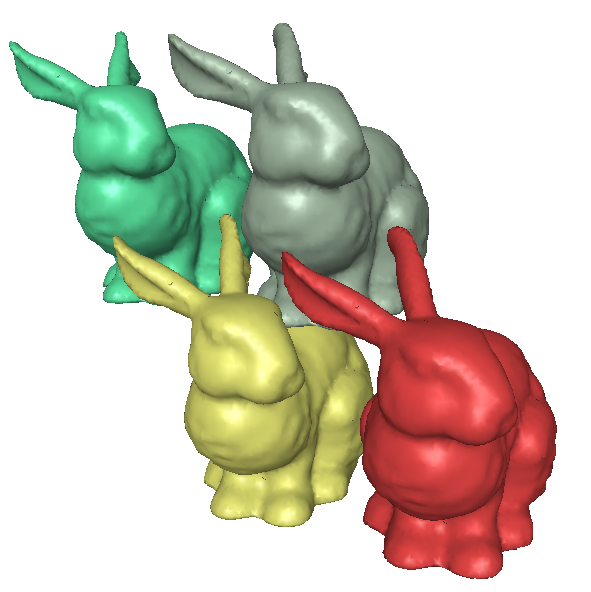
\includegraphics[width=0.98\textwidth]{filler.png} } \\
    \subfloat[][]{
      \label{fig:vertex-structure2}
      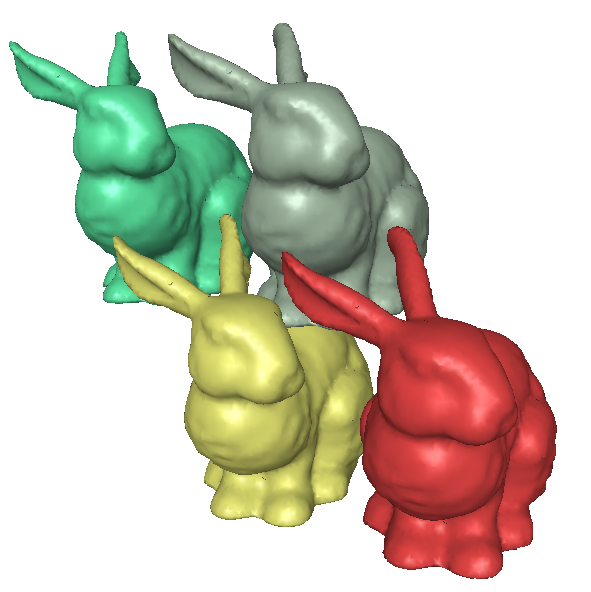
\includegraphics[width=0.98\textwidth]{filler.png} }
  \end{minipage}
  \hfill
  \begin{minipage}{0.43\columnwidth}
    \subfloat[][]{
      \label{fig:visible-vertices}
      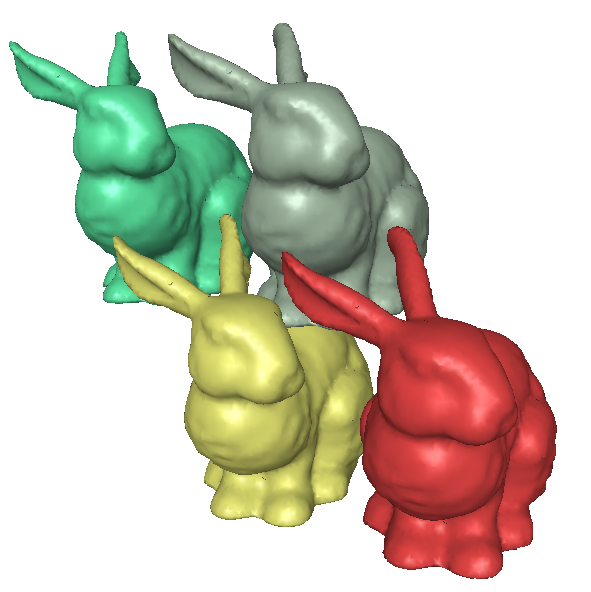
\includegraphics[width=0.98\textwidth]{filler.png} }
\end{minipage}
  \caption{\red{Quadtree (octree in 3D) cell} representation.
    \protect\subref{fig:vertex-structure1} In two dimensions, a \red{quadtree} cell is defined by four vertices.  Each vertex maintains references to its neighbors \red{with the \textit{nbrs} array}.  Two intersecting objects are shown in red and yellow.
    \protect\subref{fig:vertex-structure2} When a cell is subdivided, vertices are added and each vertex's neighbor references are updated.
    \protect\subref{fig:visible-vertices} $v$ is shaded and vertices that are visible from $v$ are circled.  A vertex $w$ is visible from $v$ if $w$ is a neighbor of $v$ or if the line segment $\overline{vw}$ has no intersections with any octree cell boundaries.}
%  \label{fig:visible-vertices}
  \label{fig:2d-octree-diagram}
\end{figure}

%\old{Our data structure does not explicitly encode a hierarchy.}
Our adjacency structure is amenable to our most important operations, which are to find an edge neighbor for the \texttt{SHOULD\_SUBDIVIDE} predicate, and finding visible vertices for the wavefront propagation.  Finding an edge neighbor is $\BigO{1}$ with our octree representation.  Gargantini's~\shortcite{gargantini1982effective} data structure has logarithmic neighbor finding, and Frisken and Perry's~\shortcite{frisken2002simple}, which has fast neighbor finding like ours, requires significant extra storage.  Computational complexity of finding visible vertices is asymptotically equal to the number of visible vertices and is discussed in Section \ref{sec:distance-transform}.  Our nonhierarchical representation is not suitable for general purposes, however, because the point location operation is $\BigO{N}$.  If the need for point location arises, then our data structure can be converted to a traditional hierarchical representation in $\BigO{N\log{N}}$ time.

%Both operations are $O(1)$ with our octree representation.  Other representations include Gargantini's~\shortcite{gargantini1982effective} which has logarithmic neighbor finding, and Frisken and Perry's~\shortcite{frisken2002simple}, which has very fast neighbor finding like ours, but requires significant extra storage.  Of course, our point location operation is an expensive $O(n)$, but we have no need for it.

%\old{We do not store a vertex's spatial position, which results in memory savings of three floating point values per vertex.  Transient position information is computed as needed during octree construction or traversals, when position of a neighboring vertex is available on the call stack.}

%\old{In addition to the octree data structure, our octree construction differs from previous methods in our predicate for deciding whether to subdivide a cell.}
Previous algorithms ensure that object features are resolved well by subdividing all nonempty cells up to a maximum level.  More sophisticated feature resolution predicates have also been used (e.g., the bilinear interpolation test of Frisken \etal~\shortcite{frisken2000adaptively}). Our subdivision predicate is different in that we are primarily interested in resolving between objects. \red{Define a face-neighbor of cell $c$ to be a cell that shares a face with $c$.} The predicate \texttt{SHOULD\_SUBDIVIDE(c)} works as follows.  Subdivide $c$ if (1) $c$ intersects more than one object, or (2) a face-neighbor of $c$ intersects with a different object. Test (1) ensures that every leaf cell after construction will intersect at most one object, and test (2) ensures that objects will be separated from each other by at least one empty buffer cell.  One advantage of \texttt{SHOULD\_SUBDIVIDE(c)} is that octree complexity becomes independent of object complexity.  As shown in Figure \ref{fig:2d-6}, even object self-intersections or nonmanifold points have no effect on octree depth, whereas the octree would be fully subdivided in those areas if using a conventional subdivision predicate.

\begin{figure}
  \centering
  \subfloat[][]{
    \label{fig:2d-6}
    \begin{tikzpicture}
      \node[anchor=south west,inner sep=0] at (0,0) {
        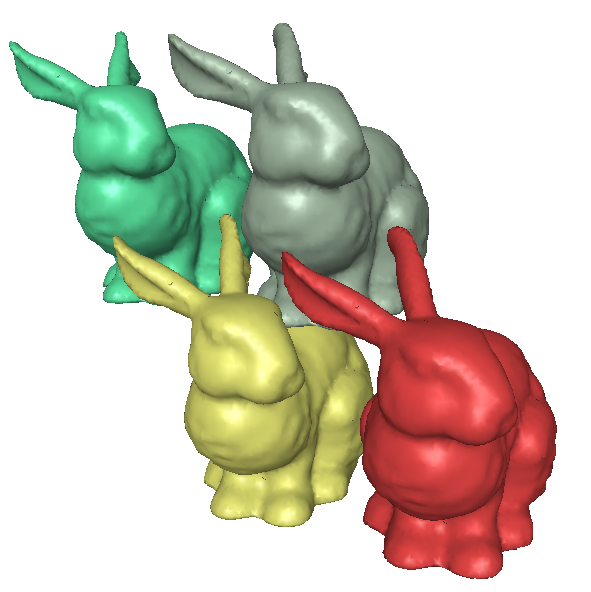
\includegraphics[width=0.31\columnwidth]{filler.png}};
      \draw [very thick,->] (2.55,1.48) -- (2.15,1.48);
      \draw [very thick,densely dotted,->] (0.6,0.9) -- (1.0,0.6);
    \end{tikzpicture}
  }
  \subfloat[][]{
    \label{fig:2d-7}
    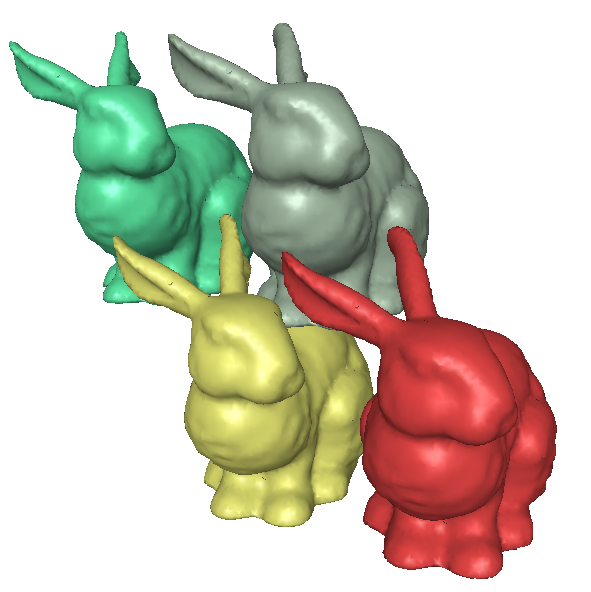
\includegraphics[width=0.31\columnwidth]{filler.png} }
  \subfloat[][]{
    \label{fig:2d-4}
    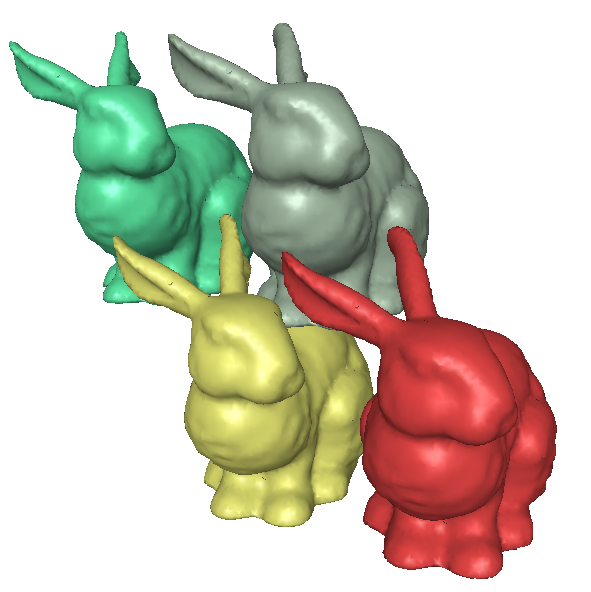
\includegraphics[width=0.31\columnwidth]{filler.png} }
  \caption{Quadtree, GVD, and distance field of intersecting, embedded, and nonmanifold 2D objects.
    \protect\subref{fig:2d-6} The quadtree is subdivided only far enough so that there is a one cell buffer between objects and so that ambiguous cells are resolved.  Object self-intersections and nonmanifold points have no effect on quadtreetree depth (solid arrow), but intersections between objects are subdivided to the maximum level (dotted arrow).
    \protect\subref{fig:2d-7} Computed GVD.
    \protect\subref{fig:2d-4} The distance field computed from the quadtree vertices.
  }
  \label{fig:predicate}
\end{figure}

%We have two options for predicates to use in deciding whether to subdivide a cell.  The first is for GVD computation.  Given a cell $c$, subdivide if (1a) $|\{S_i|c \cap S_i \ne \emptyset \}| > 1$ (if the cell intersects more than one object), or (1b) $n \in nbrs(c) \cap S_j \ne \emptyset, j \ne i$ where $nbrs(c)$ is the set of edge-neighbors of $c$ (if an edge-neighbor of $c$ intersects with a different object). Test (1a) ensures that every leaf cell after construction will intersect at most one object, and test (1b) ensures that objects will be separated from each other by at least one empty buffer cell.
%
%The second predicate is for use in building a distance field suitable for distance queries at arbitrary points and ensures that object features are well-resolved (figure \ref{fig:field-interp}).  The simplest predicate is to subdivide if the cell is nonempty up to a maximum level.  More sophisticated feature resolution predicates can be used (e.g. the bilinear interpolation test of \cite{frisken2000adaptively}).

%-----------------------------------------------------------
% Distance transform
%-----------------------------------------------------------
\section{Distance transform}
\label{sec:distance-transform}
%We compute the distance field using a novel wavefront distance transform that is similar in spirit to that of \cite{breen19983d}, with the fundamental difference being that we compute using an octree rather than a uniform grid.
Our distance transform is inspired by that of Breen \etal~\shortcite{breen19983d}, with the fundamental difference being that we compute using an octree rather than a uniform grid.  Each octree vertex has two properties -- a label and a closest point.
%An octree cell $c$ is said to be empty if $c \cap S = \emptyset$.
An octree vertex is empty if all incident cells are empty. Define the euclidean distance between two points $\dist(a,b)$ to be infinity if either $a$ or $b$ is \texttt{null} and let $\{S_i\}$ be the set of objects intersecting octree cells incident to a vertex $v$. The two main steps of distance computation are initialization of nonempty vertices and wavefront expansion.  Algorithm \texttt{COMPUTE\_DISTANCES} comprises both steps.

%Define the euclidean distance between two points $\dist(a,b)$ to be infinity if either $a$ or $b$ is \texttt{null}.  Let $\{S_i\}$ be the set of objects intersecting octree cells incident to a vertex $v$.

\algorithmspace
\begin{algorithm}
  \DontPrintSemicolon
%  \LinesNumbered
  \KwIn{Octree}
  \BlankLine
  \tcp{Initialization}
  \ForEach{vertex v in Octree}{
    \If{v is nonempty}{
      point[v] := closest point on $\{S_i\}$ to v\;
      label[v] := $i$\;
    }
    \Else{
      point[v] := null\;
    }
%    dist[v] := $\dist(v, point[v])$\;
  }
  V := the set of all vertices in Octree\;
  \tcp{Wavefront expansion}
  \While{V is not empty}{
%    v := vertex in V with minimum $|$v-point[v]$|$\;
    v := vertex in V with minimum $\dist(v, point[v])$\;
    remove v from V\;
    \ForEach{visible vertex a from v}{
      \If{$\dist(a, point[v]) < \dist(a, point[a])$}{
        point[a] := point[v]\;
        label[a] := label[v]\;
        reorder a in V\;
      }
    }
  }
\caption{COMPUTE\_DISTANCES}
\label{alg:compute-distances}
\end{algorithm}
\algorithmspace

Algorithm \texttt{COMPUTE\_DISTANCES} initializes the point assignments of nonempty vertices (Figures \ref{fig:wavefront6} and \ref{fig:wavefront2}). All closest points $point[v]$ (ties are broken arbitrarily) are stored as an array and each vertex maintains an index into the array, taking advantage of the fact that roughly half of computed closest points are shared among multiple vertices.  The closest points are computed exactly: if $\alpha(v)$ is the distance from $v$ to its closest neighbor, then only surface points in cells within $\sqrt{D} \alpha(v)$ of the vertex need be searched, making the loop an $\BigO{N + M}$ operation where $N$ is the number of octree leaf cells and $M$ is a measure of object complexity (e.g., number of triangles).  All octree cells are then added to the priority queue, an $O(N)$ or $O(N \log{N})$ operation, depending on the type of heap used for the queue.  It then iterates over vertex priority queue \texttt{V} in multiple expanding wavefronts, which are similar in behavior to Dijkstra shortest-cost path wavefronts in that the priority queue is sorted on distance to the nearest object.  The vertex $v$ at the front of the queue is the closest vertex to an object among all vertices in the queue, modulo an error term discussed below.  The assigned closest point $p$ is pushed to all vertices that are visible from $v$.  A vertex $w$ is visible from $v$ if $w$ is a neighbor of $v$ or if the intersection of the line segment $\overline{vw}$ with the edges of the octree is empty (Figure \ref{fig:visible-vertices}). Visible vertices are found efficiently using our vertex adjacency data structure.  In 2D, a simple walk around the cell is sufficient.  For example, in Figure \ref{fig:visible-vertices}, a walk is done beginning from vertex $v$ in the positive $x$ direction.  At each vertex, the walk turns left if possible, otherwise it continues forward.  Once the walk returns to $v$, the visible vertices in the upper-right cell are found, and walks are performed for the other three cells.  The complexity of the walk is $O(m)$, where $m$ is the number of visible vertices.

The number of vertices that are visible from $v$ is dependent on gradation.  Let $c_1$ and $c_2$ be adjacent cells, and let $L(c)$ be the octree level of cell $c$.  Without loss of generality, let $L(c_1) > L(c_2)$.  Gradation between adjacent cells $c_1$ and $c_2$ is defined to be $L(c_1) - L(c_2)$.  Let $g$ be the maximum gradation of any two adjacent cells.  Then the number of visible vertices is $O(2^{g(D-1)})$.  To see this, consider the 2D vertex in Figure \ref{fig:visible-vertices}.  Let the upper-right cell in the figure be cell $c$.  $v$ has two ``opposite'' edges through cell $c$, where an opposite edge is one that is not incident to $v$.  $v$ has four incident cells, for a total of eight opposite edges.  Let each incident cell be maximally graded, such that each opposite edge is incident to $2^g$ cells.  Then there are $(8)(2^{g(D-1)}) = O(2^g)$ visible vertices.  Derivation in the 3D case is similar.  If the number of visible vertices becomes a significant factor in practice, then the octree can be constructed with bounded gradation (similar to the approach of Strain~\shortcite{strain1999fast}), thereby bounding the number of visible vertices with a constant.
%If cells adjacent to $c$ are all $g$ levels down from $c$, then there are...

\begin{figure}
  \centering
  \subfloat[][]{
    \label{fig:wavefront5}
    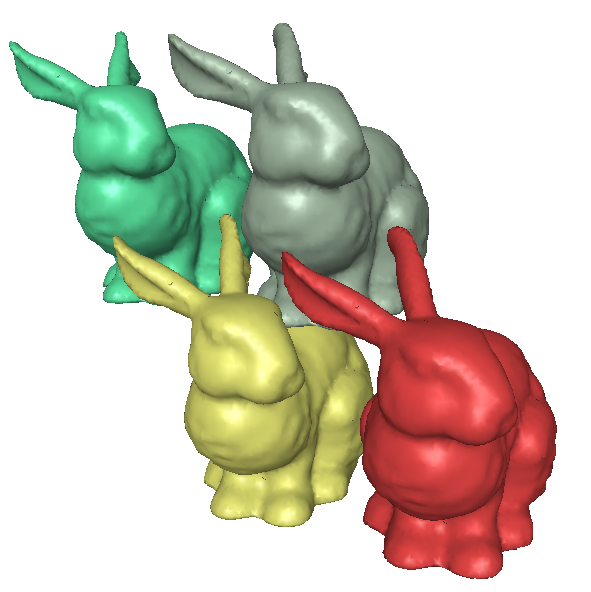
\includegraphics[width=0.32\columnwidth]{filler.png} }
  \subfloat[][]{
    \label{fig:wavefront6}
    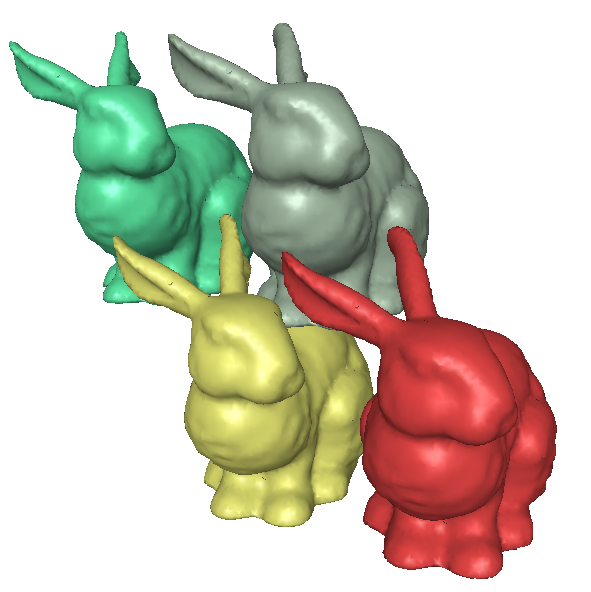
\includegraphics[width=0.32\columnwidth]{filler.png} }
  \subfloat[][]{
    \label{fig:wavefront7}
    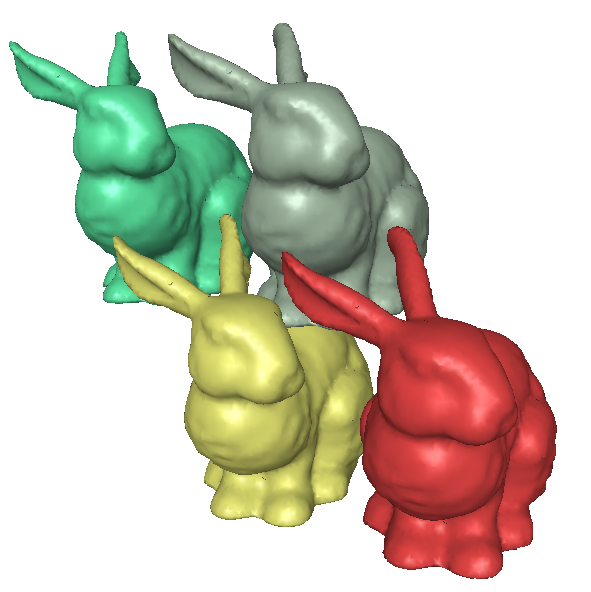
\includegraphics[width=0.32\columnwidth]{filler.png} } \\
  \subfloat[][]{
    \label{fig:wavefront2}
    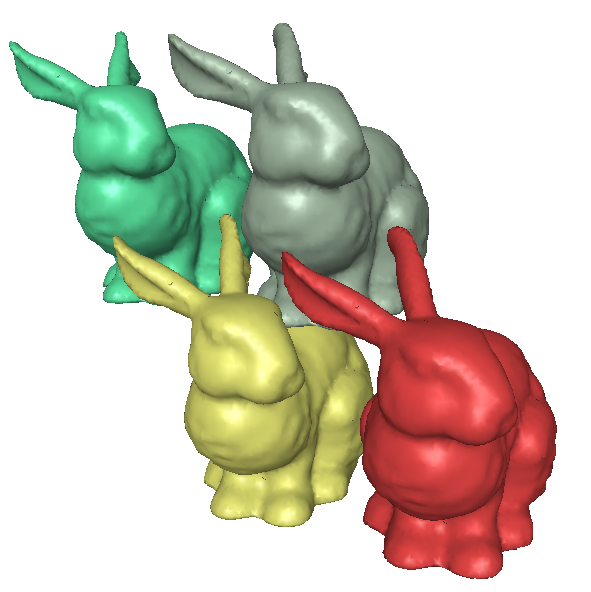
\includegraphics[width=0.32\columnwidth]{filler.png} }
  \subfloat[][]{
    \label{fig:wavefront4}
    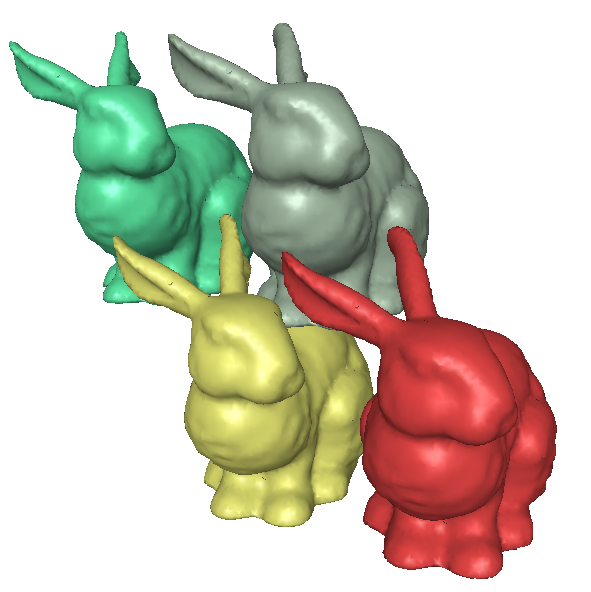
\includegraphics[width=0.32\columnwidth]{filler.png} }
  \subfloat[][]{
    \label{fig:wavefront6-gvd}
    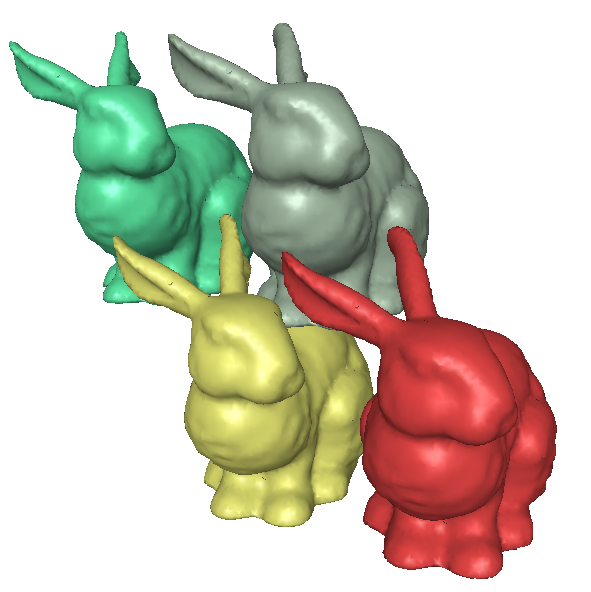
\includegraphics[width=0.32\columnwidth]{filler.png} }
  \caption{Wavefront expansion.
    \protect\subref{fig:wavefront5} Portions of the surfaces of two objects. Assign every nonempty vertex an exact closest point and add the vertex to the wavefront priority queue.
    \protect\subref{fig:wavefront6} Pop the top priority vertex (dotted circle) and push its closest point to its neighbors (circle).
    \protect\subref{fig:wavefront7} Next iteration.
    \protect\subref{fig:wavefront2} Initialized wavefront (as in \protect\subref{fig:wavefront6}).
    \protect\subref{fig:wavefront4} Expanded wavefront.  Green lines connect quadtree vertices to computed closest points.
    \protect\subref{fig:wavefront6-gvd} The GVD is shown in red.
  }
  \label{fig:wavefront}
\end{figure}

Our algorithm approximates distances on empty vertices, and our empirical tests suggest an error bound of $\frac{\e(v)}{\d(v)} \le \frac{1}{2}$, where $e(v)$ is the error at a vertex $v$ and $\d(v)$ is the distance from $v$ to the nearest point on $S$, implying that the distance transform is a $\frac{3}{2}$-approximation.  The error occurs because only closest points assigned in the wavefront initialization are propagated in the wavefront expansion.  Distance transform time complexity is $O(N+M)$ for the initialization step, $\le O(N\log{N})$ for the priority queue initialization, and $O(2^{g(D-1)}N\log{N})$ for the wavefront expansion, where the reordering of $a$ in $V$ provides the $\log{N}$ factor.  Thus, total time complexity of the transform is $O(2^{g(D-1)}N\log{N} + M)$, or $O(N\log{N} + M)$ if gradation is bounded by a constant.

% Our complexity bound highlights an advantage of decoupling octree construction and distance computation.  The top-down approaches of \cite{strain1999fast} and \cite{frisken2000adaptively} compute exact distances at each octree level for $\BigO{LF}$ where $L$ is the maximum octree level.

%\paragraph{Distance field}
%\texttt{COMPUTE\_DISTANCES} finds distances on quadtree vertices. This labeled subdivision data structure can be used as a distance representation.  That is, given any point we can quickly find an approximation of its distance from its closest site. If we desire to query our data structure for distances at arbitrary points (figure \ref{fig:field-interp}) we should use the feature resolution predicate (section \ref{sec:build-octree}) during octree construction and the octree should be stored as a hierarchy, which is better suited to point location queries (i.e., given a point $p$, find the octree leaf cell that contains $p$).  The octree can either be stored hierarchically at the outset, requiring changes to the octree construction implementation, or it can be converted to a hierarchy from the adjacency representation.
%
%The typical approach to computing the distance at a point given an ADF is to interpolate using distances of nearby vertices \cite{strain1999fast,frisken2000adaptively}. This is advantageous in that vertices need store only a distance and not the actual closest point, and the distance field will be $C^0$ continuous.  However, distance extrema will be limited to the octree vertices.  Our approach is the following: given a point $p$ and its containing leaf octree cell $c$, choose the closest point among the closest points of vertices on $c$.  That is, $point[p] = \argmin_{point[v \in c]} \dist(p, point[v])$.  While the distance field is not continuous, the benefit is that distance extrema in cell interiors can be found.

Although not designed specifically to do so, our distance-assigned octree vertices can be used to compute distance values of arbitrary points in the domain.  Given a point $p$ and its containing leaf octree cell $c$, choose the closest point among the closest points of vertices on $c$.  That is, $point[p] = \argmin_{point[v \in c]} \dist(p, point[v])$. The assigned distance is $|point[p]-p|$.  See Figure \ref{fig:2d-4} for a distance field example.
% We note that while the distance fields computed by previous approaches \cite{strain1999fast,frisken2000adaptively} are continuous, ours is not.
% While the distance field is not continuous, the benefit is that distance extrema in cell interiors can be found.

%-----------------------------------------------------------
% Resolve ambiguities
%-----------------------------------------------------------
\section{Resolve ambiguities}

\newcommand{\vlabel}{\mathscr{L}}

%Our distance function is built over a discretized space that can potentially yield ambiguities in the topology of the GVD.  We call an octree cell ambiguous if the topology of the GVD in the cell is ambiguous.  We test for cell ambiguity as follows. 0- and 1-dimensional cells are unambiguous.  Let $G_c$ be a restriction of the octree vertex graph $G$ to cell $c$.  Collapse all edges in $G_c$ that have endpoints with identical labels.  Call the new graph $\overline{G_c}$. A $(D>1)$-dimensional cell $c$ is unambiguous if $\overline{G_c}$ is a clique and all $D-1$ faces are unambiguous.  See Figure \ref{fig:ambiguous}.  Ambiguous cells are subdivided recursively until the ambiguity is resolved or a threshold level is reached (Figure \ref{fig:bisector-ambiguity}).

Our distance function is built over a discretized space that can potentially yield ambiguities in the topology of the GVD.  We call an octree cell ambiguous if the topology of the GVD in the cell is ambiguous.  We test for cell ambiguity as follows. Let $G$ be an embedded graph with vertices and edges corresponding to octree vertices and edges, respectively.  Let $G_c$ be the intersection of $G$ with octree cell $c$. See Figure \ref{fig:ambiguous}. Collapse all edges in $G_c$ that have endpoints with identical labels.  Call the new graph $\overline{G_c}$. Cell $c$ is unambiguous if $\overline{G_c}$ is a $(\le D)$-dimensional simplex.
%The proof is that every generalized Voronoi cell (GVC) in $c$ is incident with every other GVC in $c$ because every vertex in a simplex shares an edge with every other vertex.
\begin{proof}
Let $M=\{M_i\}$ be the set of generalized Voronoi cells (GVCs) that intersect with $c$.  Because every vertex in a simplex shares an edge with every other vertex, the topology of the GVD in $c$ is given by $M_i \cap M_j \cap c \ne \emptyset$.
\end{proof}

Ambiguous cells are subdivided recursively until the ambiguity is resolved or a threshold subdivision level is reached (Figure \ref{fig:bisector-ambiguity}).  If the threshold is reached then the topology is decided as described in Section \ref{sec:bisector}.

\begin{figure}
  \centering
  \fbox{\subfloat[][$G_x$]{
    \label{fig:ambiguous3}
    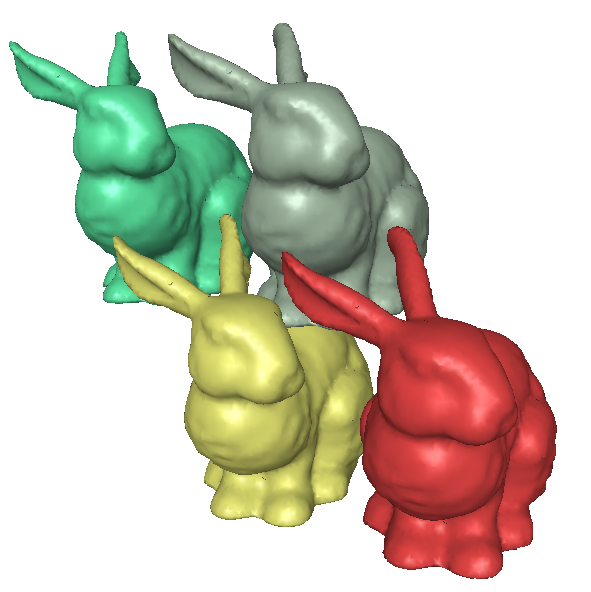
\includegraphics[width=0.16\columnwidth]{filler.png}
  }
  \subfloat[][$\overline{G_x}$]{
    \label{fig:ambiguous4}
    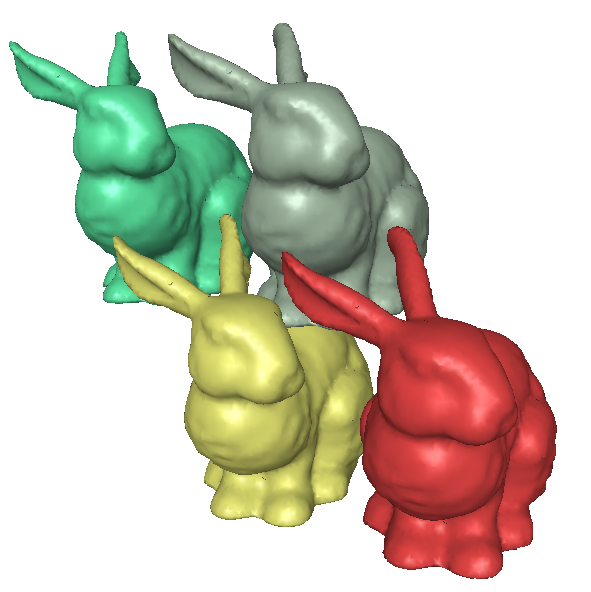
\includegraphics[width=0.16\columnwidth]{filler.png}
  }
  \subfloat[][$\overline{G_x}$]{
    \label{fig:ambiguous5}
    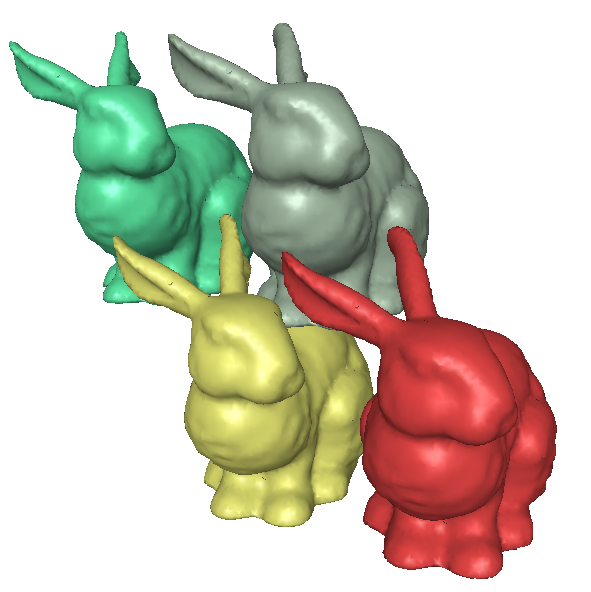
\includegraphics[width=0.16\columnwidth]{filler.png}
  }}
  \fbox{\subfloat[][$G_y$]{
    \label{fig:ambiguous1}
    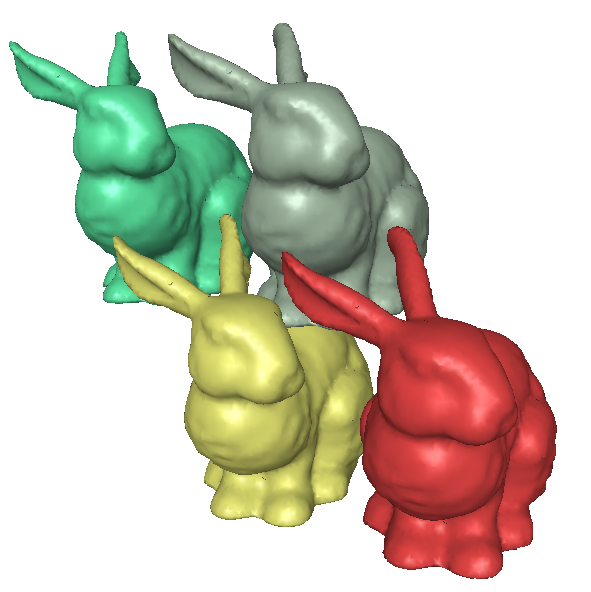
\includegraphics[width=0.16\columnwidth]{filler.png}
  }
  \subfloat[][$\overline{G_y}$]{
    \label{fig:ambiguous2}
    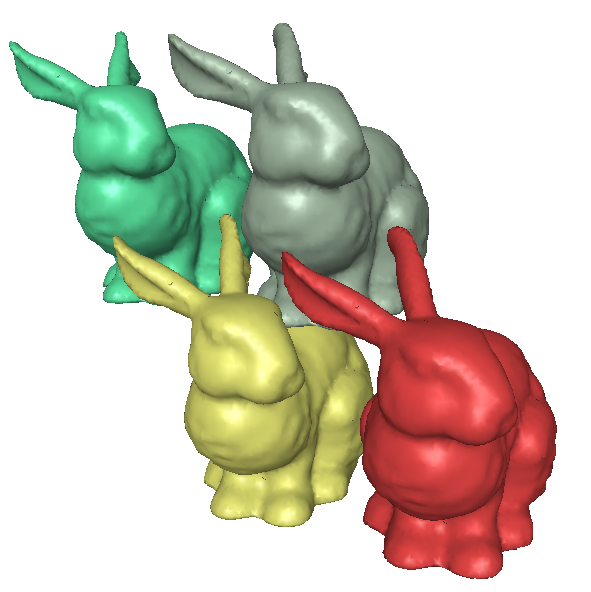
\includegraphics[width=0.16\columnwidth]{filler.png}
  }}
  \caption{
Ambiguous cells are detected by collapsing edges with identically labeled vertices.
    \protect\subref{fig:ambiguous3} Cell $x$ is ambiguous because $\overline{G_x}$ is not a simplex.
    \protect\subref{fig:ambiguous4}-\protect\subref{fig:ambiguous5} Two possible GVD topologies in cell $x$ are shown.
    \protect\subref{fig:ambiguous1} Cell $y$ is unambigous.
    \protect\subref{fig:ambiguous2} Simplex $\overline{G_y}$ induces a unique GVD topology.
  }
  \label{fig:ambiguous}
\end{figure}

\begin{figure}
  \centering
  \subfloat[][]{
    \label{fig:bisector-ambiguity0}
    \begin{tikzpicture}
      \node[anchor=south west,inner sep=0] at (0,0) {
        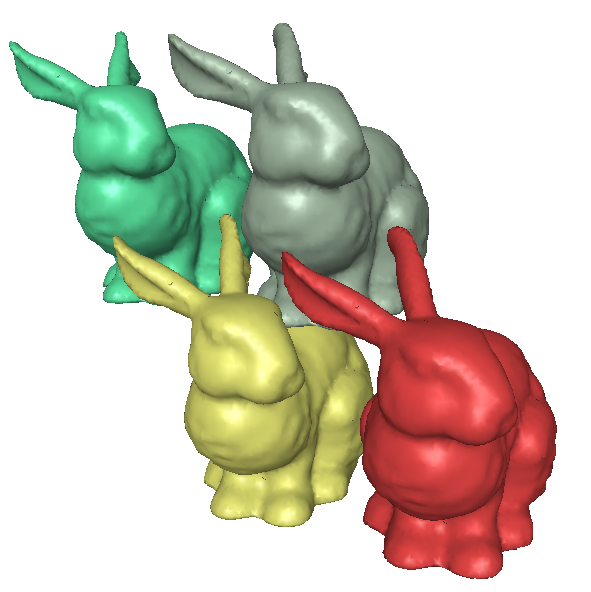
\includegraphics[width=0.3\columnwidth]{filler.png}};
      \draw [red,thick,->] (2.2,1.57) -- (1.9,1.57);
      \draw [red,thick,->] (2.2,1.57) -- (2.2,1.27);
    \end{tikzpicture}
  }
  \hspace{1cm}
  \subfloat[][]{
    \label{fig:bisector-ambiguity1}
    \begin{tikzpicture}
      \node[anchor=south west,inner sep=0] at (0,0) {
        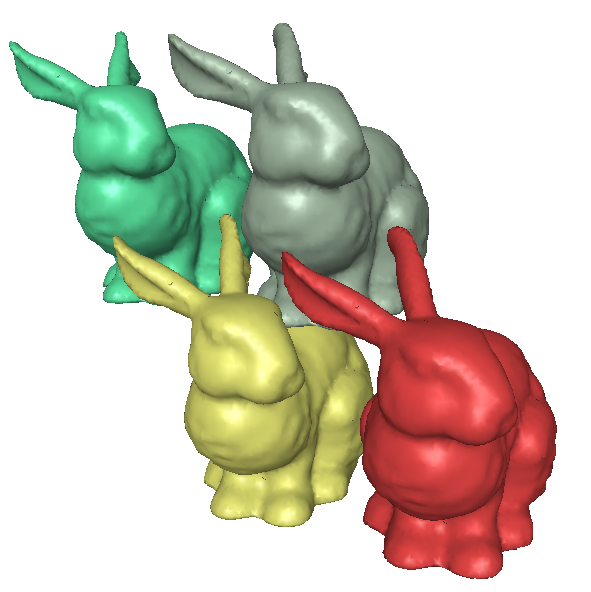
\includegraphics[width=0.3\columnwidth]{filler.png}};
    \end{tikzpicture}
  }
  \caption{The effect of ambiguous cells and how they are removed.
    \protect\subref{fig:bisector-ambiguity0} The cells indicated by the arrows are ambiguous, causing the GVD to be topologically incorrect.
    \protect\subref{fig:bisector-ambiguity1} The ambiguities are resolved by recursive subdivision.}
  \label{fig:bisector-ambiguity}
\end{figure}

%-----------------------------------------------------------
% Compute GVD surface
%-----------------------------------------------------------
\section{Compute GVD surface}
\label{sec:bisector}

With the distance function in place we compute the generalized Voronoi diagram, or the set of all points that have at least two closest points with differing labels, \red{using an algorithm inspired by marching cubes \cite{lorensen1987marching}}. We store the GVD as sets of \red{simplices (i.e. line segments in 2D, triangles in 3D)}, one set per object, representing the boundary of the generalized Voronoi cell (GVC) for that object.  Each simplex is stored twice, once for each GVC it borders, oriented toward the inside of the GVC.

We first compute which edges of the octree intersect the GVD by considering each octree edge $e$ with endpoint vertices $(e_0, e_1)$.
%$e_{j \in \{0,1\}}$.
Let $\vlabel(v)$ be the label of octree vertex $v$.  If $\vlabel(e_0) \ne \vlabel(e_1)$, then $e$ intersects the GVD.  Let $a=point[e_0]$ and $b=point[e_1]$.  Assume without loss of generality that $e$ is aligned with the x-axis.  Cases of alignment with $y$ and $z$ are similar.  We seek point $p=(x,y,z) \in e$ such that $\dist(a,p)=\dist(b,p)$ (see Figure \ref{fig:compute-q}). In our euclidean setting this reduces to
\begin{equation}
x = \frac{2y(a_y-b_y)+2z(a_z-b_z)+b^Tb - a^Ta}{2(b_x-a_x)}
\end{equation}

\begin{figure}
  \centering
  \begin{tikzpicture}
    \node[anchor=south west,inner sep=0] at (0,0) {
      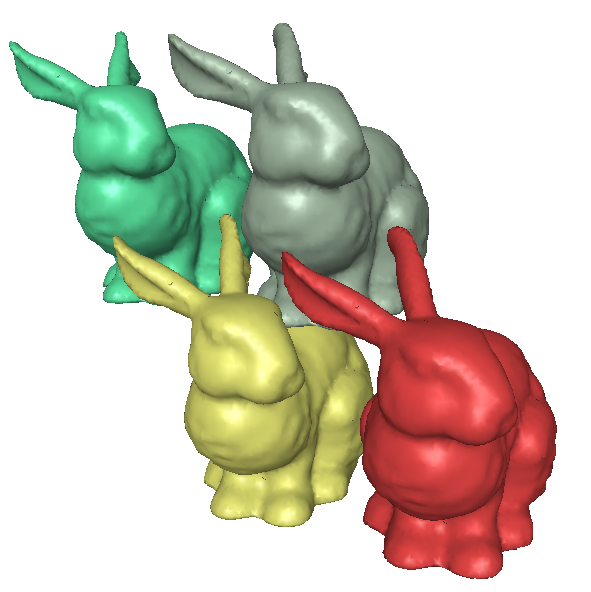
\includegraphics[width=0.5\columnwidth]{filler.png}
    };
    \node[] at (0.9,1.5) {$a$};
    \node[] at (3.2,2.05) {$b$};
    \node[] at (1.8,1.03) {$e$};
    \node[] at (2.43,0.6) {$p$};
  \end{tikzpicture}
%  \caption{Computing the intersection of the bisector of objects $a$ and $b$ with a quadtree edge.}
  \caption{Computing the intersection of the GVD with quadtree edge $e$. $a$ and $b$ are closest points on objects, and $p$ is the intersection of edge $e$ with the GVD.
    %The GVD locally bisects points $a$ and $b$.
  }
  \label{fig:compute-q}
\end{figure}

Once all edge bisectors for a cell are calculated, we fit \red{simplices} (Figure \ref{fig:bisector}). Suppose bisector $p_i$ lies on edge $e^i$. We connect bisector points on a 2D face $f$ by creating line segments between each bisector $p_i \in f$ and the centroid of all face bisectors $r_f = \sum p_i / |\{p_i\}|$.  If the 2D cell is unambiguous there will be at most three bisectors.  In the case that the cell is subdivided to the threshold level without resolving ambiguity then the centroid $r_f$ becomes an interface to four or more generalized Voronoi cells. Other approaches to ambiguity resolution include \cite{natarajan1994generating,nielson1991asymptotic,sohn2007topology}.   We label each line segment by the labels of the vertices adjacent to $p_i$, that is,  $\vlabel(p_i) = \alpha\beta$ where $\vlabel(e^i_0) = \alpha$ and $\vlabel(e^i_1) = \beta$. \red{If we are computing a 2D GVD then we are done.}

\red{In 3D,} given a cell $c$, we first find the line segment complex of each 2D face $c$ using the 2D algorithm and union all segments into a set $C_c$.  We then form triangles from each segment in $C_c$
%$h \in C_c$
to the 3D centroid $r_c$ of the bisectors (Figure \ref{fig:bisector3}).  Triangle $t_i$ has vertices $(p_i, r_f, r_c)$. We maintain a set $T_{\alpha}$ of triangles assigned to the GVC of the object with label $\alpha$.
%We know that triangles with the same vertices as $t_i$ must be added to $T_{\alpha}$ and $T_{\beta}$ since $\vlabel(p_i) = \alpha\beta$.
To determine the orientation we use the normal $n_{t_i}$ and the vertex $v_{p_i}^{\alpha}$ adjacent to $p_i$ with label $\alpha$. If $n_{t_i} \cdot (v_{p_i}^{\alpha}-r_c) < 0$, then we invert $t_i$ before adding it to $T_{\alpha}$, and similarly with $T_{\beta}$. The resulting GVD is water tight and each GVC is orientable.

The GVD surfacing algorithm is parallelizable, as the \red{simplices} in each octree cell are computed independently of all other octree cells.

\begin{figure}
  \centering
  \subfloat[][]{
    \label{fig:bisector2}
    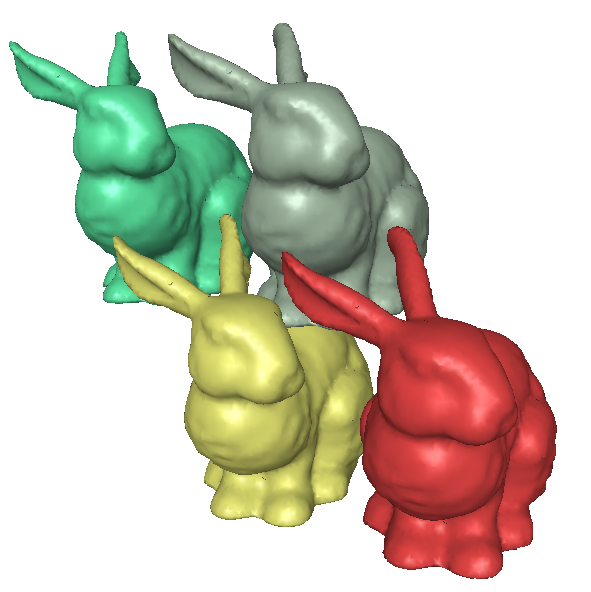
\includegraphics[width=0.4\columnwidth]{filler.png} }
  \subfloat[][]{
    \label{fig:bisector3}
    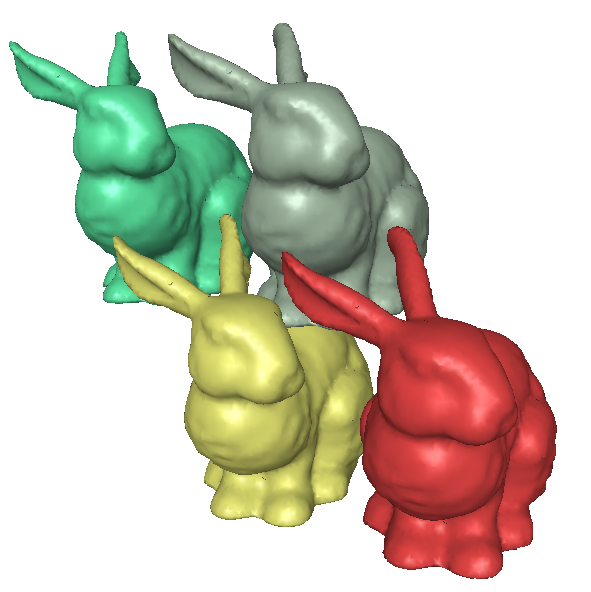
\includegraphics[width=0.4\columnwidth]{filler.png} }
  \caption{GVD surface generation.
    \protect\subref{fig:bisector2} The 2D algorithm creates GVD edges from bisectors $\{p_i\}$ to the centroid.  Each new GVD edge is given the two labels of the incident octree edge.
    \protect\subref{fig:bisector3} After finding the 2D GVD on its faces, the 3D cell fits triangles from 2D edges to the centroid.  %Each triangle is assigned to two sets of triangles, one for each label assigned to $p_i$.
  }
  \label{fig:bisector}
\end{figure}

%-------------------------------------------------------------------------------
% Results
%-------------------------------------------------------------------------------
\section{Results and applications}
Our implementation\footnote{Source code is available at \url{http://cedmav.org/research/project/33-gvds.html}.} of the algorithm supports \red{polygons and} triangulated objects, and our wavefront initialization step is implemented on the GPU using OpenCL. All tests were run on a MacBook Pro laptop with a dual-core 2.9 GHz processor, 8 GB memory, and Intel HD 4000 graphics card. Figure \ref{fig:bunny} shows our implementation of the GVD computation pipeline, and Figure \ref{fig:pipes} shows the computed GVD on a more challenging dataset.  We compare our method with other work and then show examples in three application settings: path planning, proximity queries, and exploded diagrams.

\subsection{Comparison to other methods}

Our GVD computations use commodity hardware, even on the most challenging datasets.  Uniformly gridded approaches \cite{cao2010parallel,fischer2006fast,hsieh2005simple,rong2007variants,sud2006interactive,sud2006fast,hoff1999fast,wu2008gpu,yin2011fast} require $2^{Dn}$ voxels, where $D$ is the dimension and $n$ is the number of octree levels needed to resolve objects.  Table \ref{tab:timings} shows our results on datasets that would require prohibitive numbers of voxels using uniformly gridded methods.%timings on datasets that would require between $2^{24}$ and $2^{48}$ uniformly gridded voxels.

In addition to datasets with closely spaced objects, our algorithm works on intersecting and embedded objects, nonmanifold objects, and objects with multiple connected components (see Figures \ref{fig:2d-6}, \ref{fig:2d-7}, and \ref{fig:heart}), which are not supported by Boada \etal~\shortcite{boada2008approximations}.

%\old{The sparse voxel octree method~\mbox{\shortcite{laine2011efficient}} is one of a class of algorithms that build an octree based on object surfaces \mbox{\cite{baert2013out,bastos2008gpu,crassin2009gigavoxels,lefebvre2007compressed,strain1999fast}}. The octrees are not the same as ours (sparse voxel octrees do not resolve between objects; we do not resolve object features). We include a timing and memory comparison with Laine's algorithm in Figure \ref{fig:compare} to show that our octree building algorithm is at least on par with the current state of the art.}

\red{We ran timing comparisons of our method with Laine's algorithm~\shortcite{laine2011efficient}, which is a sparse voxel octree (SVO) method \cite{baert2013out,bastos2008gpu,crassin2009gigavoxels,lefebvre2007compressed,strain1999fast}. Laine's algorithm (and other SVO methods) subdivide octree cells in areas of object complexity, whereas our algorithm subdivides in areas of inter-object proximity. In other words, previous methods model the objects, while our approach models the space between objects. Because the two methods compute different octrees, a direct timing comparison is not meaningful, so we compared the number of seconds required for each megabyte of octree. From Figure \ref{fig:compare} we see that the execution time of our algorithm is comparable to the state of the art SVO construction.}

%While part of our algorithm implementation is on the GPU (wavefront initialization and portions of the octree computation), our primary goal is to show that GVD computation using commodity hardware is possible on challenging datasets.  Uniformly gridded approaches would require $2^{Dn}$ voxels, where $D$ is the dimension and $n$ is the number of octree levels needed to resolve objects.  Table \ref{tab:timings} shows timings on datasets that would require between $2^{24}$ and $2^{48}$ uniformly gridded voxels.

%datasets where other approaches fail, rather than incremental performance improvements over previous work.  Table \ref{tab:timings} shows timings on datasets that state-of-the-art approaches fail to compute.  Uniform gridding schemes require $2^{dn}$ voxels where $d$ is the dimension and $n$ is the quadtree/octree depth.  Datasets reported in Table \ref{tab:timings} require between $2^{24}$ and $2^{48}$ uniformly gridded voxels.

%Our algorithm is designed primarily for memory savings, but it is has fast execution times as well.  We report statistics and timings in table \ref{tab:timings} for many of the examples shown in the paper.

% Memory usage:
% Vertex: 29
% Labeled point: 16
% v2b etc: 8
% total: 54
% Multiply # octree vertices by 54

% # octree vertices
%  52K ./viewer3 -l 8 ~/data/gears/gear[1-3].obj
% 170K ./viewer3 -l 12 ~/data/knife/knife-holder.obj ~/data/knife/knife[2-4].obj
% 146K ./viewer2 -l 24 ../data2/filled_ut/*.dat
% 2.8M ./viewer3 --uniform-colors -a 1 -l 8 ~/data/neuron/improved/a*.obj
% 1.3M ./viewer3 -l 8 ~/data/rice-dwarf/decimated2/n1UF2a-*.obj

% memory (54 bytes per octree cell)
%  2.8Mb ./viewer3 -l 8 ~/data/gears/gear[1-3].obj
%  9.2Mb ./viewer3 -l 12 ~/data/knife/knife-holder.obj ~/data/knife/knife[2-4].obj
% 7.9Mb ./viewer2 -l 24 ../data2/filled_ut/*.dat
% 151.2Mb ./viewer3 --uniform-colors -a 1 -l 8 ~/data/neuron/improved/a*.obj
% 70.2Mb ./viewer3 -l 8 ~/data/rice-dwarf/decimated2/n1UF2a-*.obj

\begin{table*}
  \centering
  \footnotesize{
  \begin{tabular}{l c c c c c c c}
    \toprule
    dataset & objects & object          & octree   & octree          & octree &
    GVD   & GVD             \\
            &         & $\Delta$s       & depth    & cells           & memory &
    (sec) & $\Delta$s       \\
            &         & ($\times 10^3$) &          & ($\times 10^3$) & (Mb)   &
          & ($\times 10^3$) \\
    \midrule
    % ./viewer3 -l 8 ~/data/gears/gear[1-3].obj
    Fig. \ref{fig:gears} & 3 & 7 & 8 & 54 & 3 & 0.9 & 83\\
    % ./viewer3 -l 12 ~/data/knife/knife-holder.obj ~/data/knife/knife[2-4].obj
    Fig. \ref{fig:knife} & 4 & 15 & 12 & 146 & 9 & 3.9 & 232 \\
    % ./viewer2 -l 24 ../data2/filled_ut/*.dat
    Fig. \ref{fig:path} & 470 & 5 & 24 & 158 & 8 & 2.0 & 151 \\
    % ./viewer3 --uniform-colors -a 1 -l 8 ~/data/neuron/improved/a*.obj
    Fig. \ref{fig:axons} & 448 & 4015 & 8 & 2716 & 151 & 195 & 8100 \\
    % ./viewer3 -l 8 ~/data/rice-dwarf/decimated2/n1UF2a-*.obj
    Fig. \ref{fig:mol-explode} & 35 & 1500 & 8 & 496 & 70 & 19 & 2700 \\
    \bottomrule
  \end{tabular}}
  \caption{Table of octree/GVD computation statistics and timings on datasets that are unmanageable using other methods. \red{Columns are: \emph{objects} - the number of objects in the dataset; \emph{object $\Delta$s} - the number of line segments (2D) or triangles (3D) of all objects in the dataset; \emph{octree depth} - required octree depth in order to resolve objects; \emph{octree cells} - total number of leaf octree cells; \emph{octree memory} - amount of memory used by the octree; \emph{GVD (sec)} - seconds to perform all steps of GVD computation; \emph{GVD $\Delta$s} - number of line segments (2D) or triangles (3D) in the GVD.}}
  \label{tab:timings}
\end{table*}

\begin{figure}[h]
  \centering
  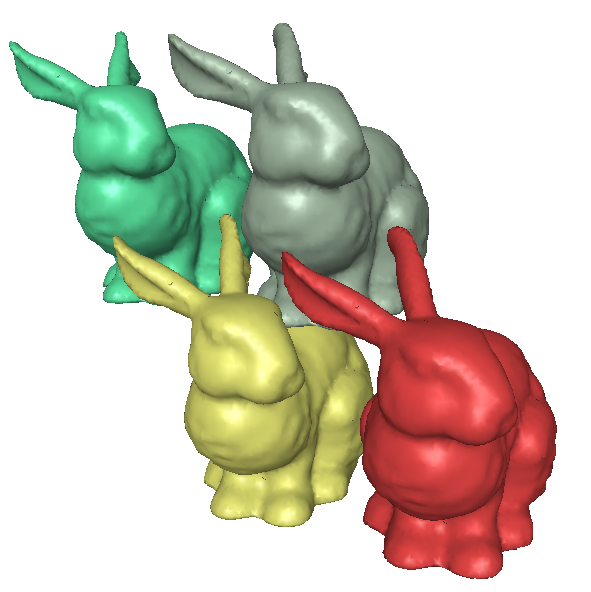
\includegraphics[width=.99\columnwidth]{filler.png}
  \caption{Comparison of our octree building to the sparse voxel octree method of Laine and Karras~\shortcite{laine2011efficient}.
    We used four datasets, each at three octree levels and compared seconds per Mb of octree memory used.
%    Our method is faster and uses less memory in almost every case.
    Laine's algorithm was run on a Windows 7 desktop with 3.5 GHz processor, 16 GB memory, and NVIDIA GeForce GTX 660 graphics card.
%  Our method is faster and uses less memory in almost every case, due to the fact that the sparse voxel octree method subdivides everywhere on the surface, whereas our approach only subdivides where object pair spacing is small.
  }
  \label{fig:compare}
\end{figure}

\begin{figure}[h]
  \centering
  \subfloat[][]{
    \label{fig:bunny1}
    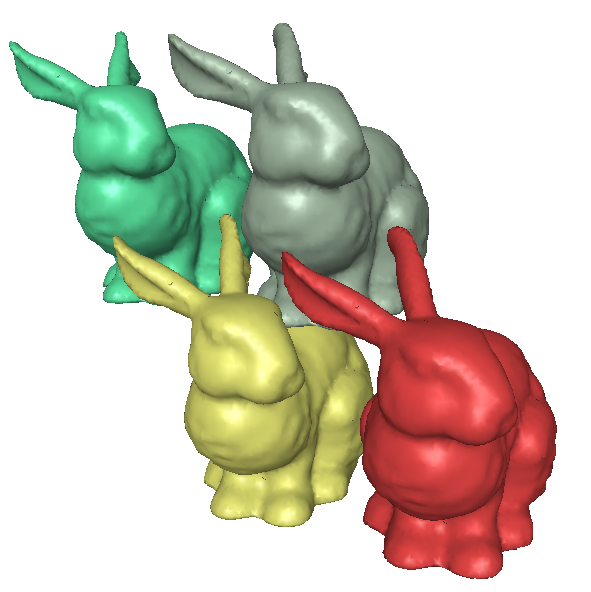
\includegraphics[width=.31\columnwidth]{bunny-4.png}
  }
  \subfloat[][]{
    \label{fig:bunny2}
    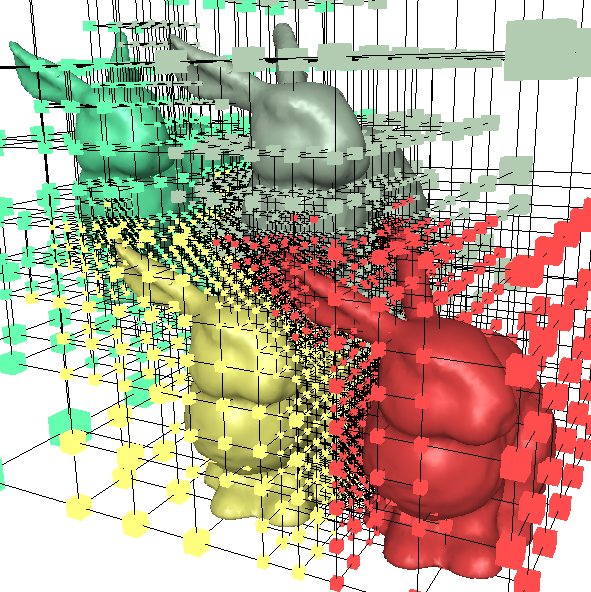
\includegraphics[width=.31\columnwidth]{bunny-5.png}
  }
  \subfloat[][]{
    \label{fig:bunny3}
    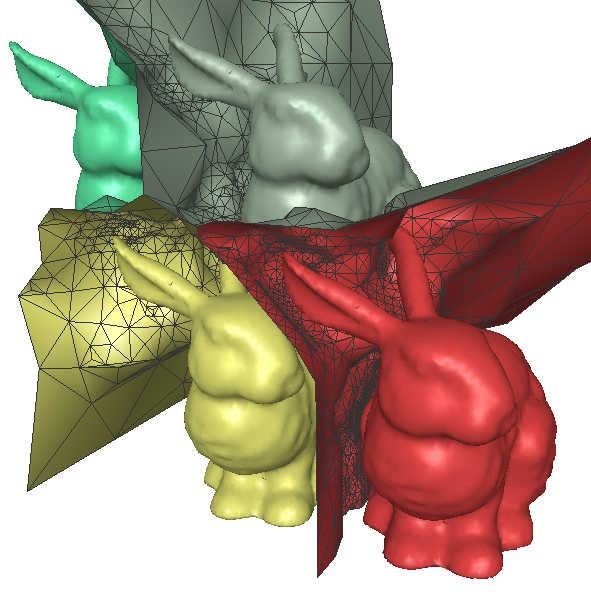
\includegraphics[width=.31\columnwidth]{bunny-6.png}
  }
  \caption{The method pipeline in 3D.
    \protect\subref{fig:bunny1} Four bunnies placed in proximity.
    \protect\subref{fig:bunny2} The octree with appropriately-labeled vertices.
    \protect\subref{fig:bunny3} The constructed GVD.
  }
  \label{fig:bunny}
\end{figure}

\begin{figure}[h]
  \centering
  \begin{tikzpicture}
    \node[anchor=south west,inner sep=0] at (0,0) {
      \begin{minipage}{0.3\columnwidth}
        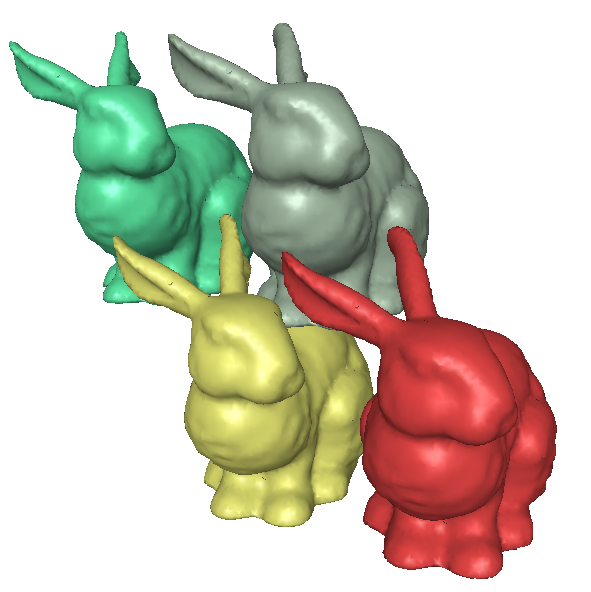
\includegraphics[trim=6cm 1cm 7cm 1cm, clip=true, height=3cm]
                        {filler.png}
      \end{minipage}
      \begin{minipage}{0.3\columnwidth}
        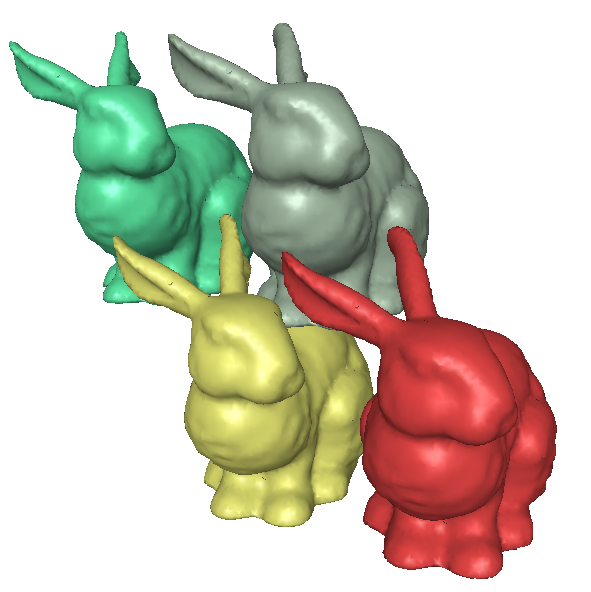
\includegraphics[trim=6cm 0cm 4cm 0cm, clip=true, height=3cm]
                        {filler.png}
      \end{minipage}
      \hspace{0.5cm}
      \begin{minipage}{0.3\columnwidth}
        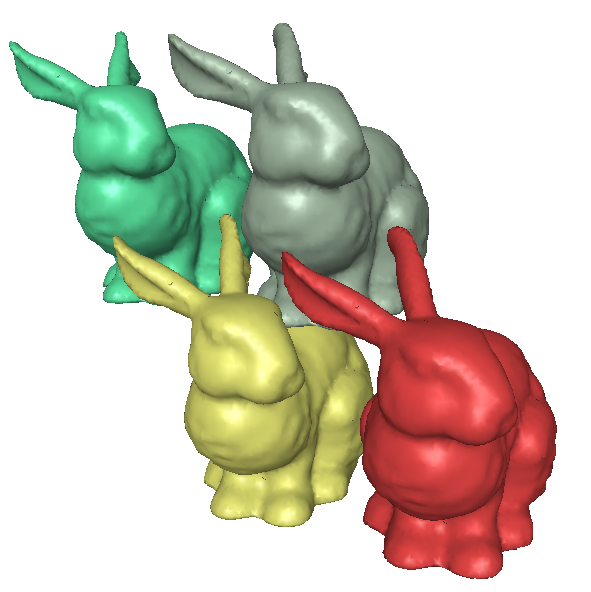
\includegraphics[trim=4cm 0cm 1cm 0cm, clip=true, width=1.9cm]
                        {filler.png} \\
                        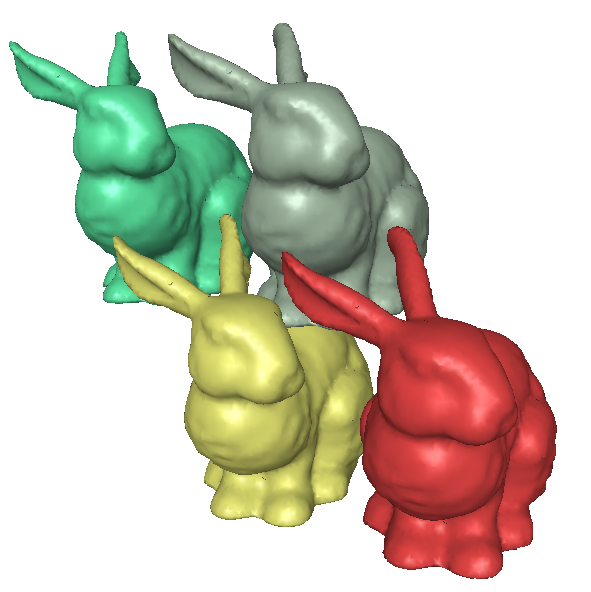
\includegraphics[trim=4cm 2.8cm 4cm 2.4cm, clip=true, width=1.9cm]
                                        {filler.png}
      \end{minipage}
    };
    % top box
    \draw[red,thick] (4.25,2.15) rectangle (4.7,2.65);
    \draw[red] (4.25,2.65) -- (5.3,3.27);
    \draw[red] (4.25,2.15) -- (5.3,1.55);
    \draw[black] (5.3,1.55) rectangle (7.2,3.27);
    % bottom box
    \draw[red,thick] (2.9,1.8) rectangle (3.6,2.2);
    \draw[red] (3.6,2.02) -- (5.3,1.5);
    \draw[red] (2.9,1.8) -- (5.3,0.02);
    \draw[black] (5.3,0.02) rectangle (7.2,1.5);
%    % top box
%    \draw[red,thick] (4.45,2.15) rectangle (4.9,2.65);
%    \draw[red] (4.45,2.65) -- (5.82,3.27);
%    \draw[red] (4.45,2.15) -- (5.82,1.55);
%    \draw[black] (5.82,1.55) rectangle (7.72,3.27);
%    % bottom box
%    \draw[red,thick] (3.1,1.8) rectangle (3.8,2.2);
%    \draw[red] (3.8,2.02) -- (5.82,1.5);
%    \draw[red] (3.1,1.8) -- (5.82,0.02);
%    \draw[black] (5.82,0.02) rectangle (7.72,1.5);

%    \draw[black,thick] (0.6,1.8) -- (2.75,4.45);
%    \draw[black,thick] (2.75,0.5) rectangle (8.25,4.47);
  \end{tikzpicture}
  \caption{A pipes dataset with 392 objects and 207K object triangles.  The octree was subdivided to level 10 for a total of 1.8m octree cells.  The GVD separates even the nuts from the bolts (upper right).
  }
  \label{fig:pipes}
\end{figure}

\begin{figure}[h]
  \centering
  \begin{tikzpicture}
    \node[anchor=south west,inner sep=0] at (0,0) {
      \subfloat[][]{
        \label{fig:heart1}
        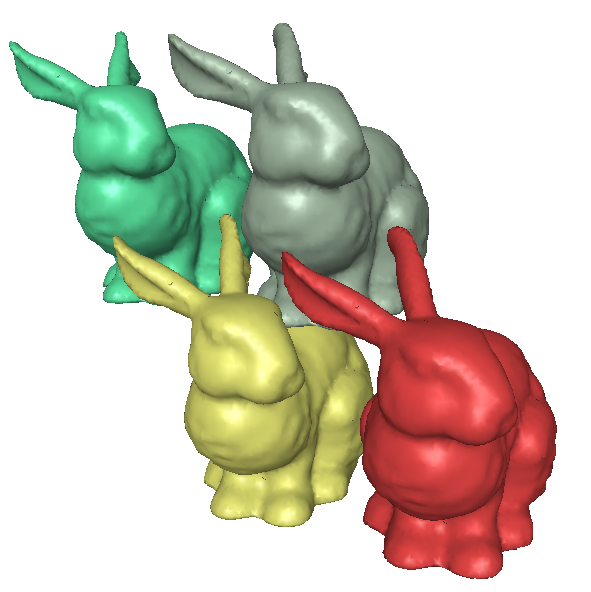
\includegraphics[trim=9cm 0cm 6cm 0cm, clip=true, height=3cm]
                        {filler.png} }
      \subfloat[][]{
        \label{fig:heart2}
        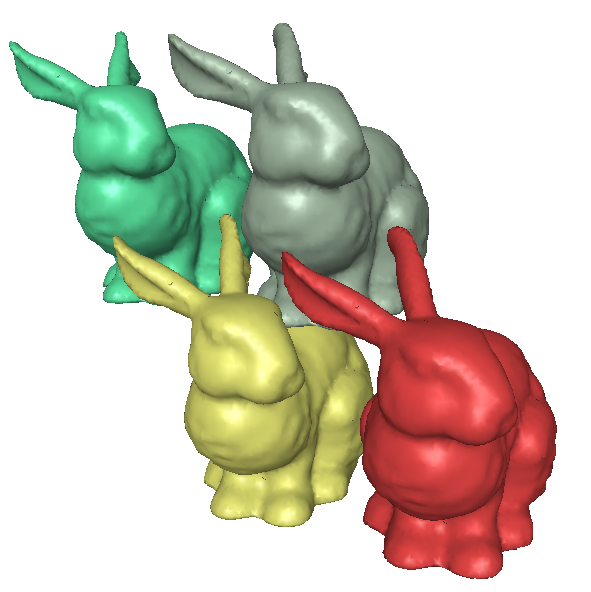
\includegraphics[trim=0cm 1cm 0.5cm 0cm, clip=true, height=3cm]
                        {filler.png} }
    };
    \draw[black,ultra thick] (0.5,0.9) rectangle (1.2,1.45);
    \draw[black,thick] (0.5,0.9) -- (2.1,0.5);
    \draw[black,thick] (0.5,1.45) -- (2.1,3.5);
    \draw[black,thick] (2.1,0.5) rectangle (6.25,3.5);
  \end{tikzpicture}
  \caption{%\red{fix image}
    Heart defibrillation dataset showing support for multiple connected components.
    \protect\subref{fig:heart1} The blue and purple objects have multiple components.
    \protect\subref{fig:heart2} The GVD naturally handles multiple components of an object.  Portions of the GVD are clipped away for visualization.
  }
  \label{fig:heart}
\end{figure}

\subsection{Path planning}
\label{sec:path-planning}

\red{Motion planning is an important application in robotics and other fields \cite{canny1988simplified,thrun1998learning,hoff2000interactive,vachhani2011mobile}. Roadmap methods of path finding \cite{masehian2007classic,raja2012optimal} retract the set of feasible movements to a lower-dimensional space, often using the Generalized Voronoi Diagram as the retraction. Once the GVD is available, a variety of methods can be used for computation of the final path, from simple graph searches \cite{hoff2000interactive,masehian2007classic} to fast marching \cite{garrido2006path}. As noted by Foskey et al \shortcite{foskey2001voronoi}, a shortcoming of this approach is the difficulty of computing the GVD.}

\red{We have augmented our GVD algorithm with a simple path finding implementation that uses Dijkstra's graph search algorithm in order to show that path planning is possible on difficult datasets. On simple datasets, our method is not competitive with uniform grid approaches \cite{hoff2000interactive,foskey2001voronoi,garrido2006path}, but our algorithm is robust on datasets with closely spaced objects, which would cause uniform grid approaches to fail. One such dataset is shown in Figure \ref{fig:path}, where we computed the GVD for 470 2D objects with object spacings that vary widely. Computation took 2.0 seconds with the quadtree reaching level 24 and 140,680 cells (a uniform grid would require $2^{48}$ pixels to resolve the closest object spacings). Our GVD algorithm could be coupled with a more sophisticated path search algorithm, such as the method proposed by Garrido et al \shortcite{garrido2006path}, for improved paths.}

\begin{figure*}
  \centering
  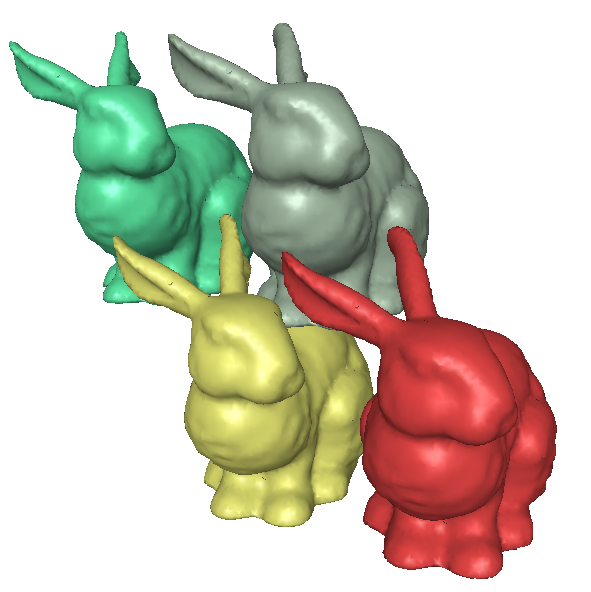
\includegraphics[width=0.8\textwidth]{filler.png}
  \caption{Path planning in 2D.  We built a quadtree over hundreds of objects ranging in size and spacing over orders of magnitude.  The quadtree reached level 24 before the closest spacings were resolved.  The shortest-cost path between two points is shown in blue.  The rightmost figure shows the quadtree in gray and GVD boundary complex in red at 80,000x magnification.}
  \label{fig:path}
\end{figure*}

\subsection{Proximity queries}
\label{sec:proximity}

\subsection{Exploded diagrams}

%-------------------------------------------------------------------------------
% Conclusions
%-------------------------------------------------------------------------------
\section{Conclusions}
We have presented and demonstrated the effectiveness of a novel generalized Voronoi diagram algorithm, which includes an octree subdivision algorithm, octree data structure, distance transform, and GVD surfacing algorithm.  We have also shown, in addition to the popular motion path planning, important applications of the GVD.  Our method opens the door to investigation of other applications that might benefit from a GVD algorithm specifically tailored to collections of objects that are closely spaced.

Our algorithm is general; our implementation supports \red{polygons and} triangulated objects, but the algorithm supports curved objects equally as well.  Our approach is particularly suited to objects for which a point-object distance computation is expensive since initialization of the wavefront is the only step that requires the point-object distance operation.

With the proven usefulness of the ordinary Voronoi diagram and the growing uses of the generalized Voronoi diagram, the algorithm presented in this paper fills a need for a practical GVD algorithm that supports previously unmanageable datasets -- those with tightly packed objects.  Interestingly, it is often applications using these very datasets that are in greatest need of the GVD.  For example, traditional path-planning is straightforward unless the objects are tightly packed; finding regions of close tolerance is unnecessary unless close tolerances, in fact, exist.  These applications and others can now be more fully explored with the availability of our adaptive GVD algorithm.

%-------------------------------------------------------------------------------
% Acknowledgements
%-------------------------------------------------------------------------------
\section*{Acknowledgements}
Thanks to Kristen Harris for use of the neuronal data and Jonathan Bronson for the heart data. The work of JE and VP was supported in part by NSF IIS-1314896, NSF ACI-0904631, DOE/NEUP 120341, DOE/UV-CDAT DESC0006872, DOE/Codesign P01180734, DOE/SciDAC DESC0007446, DOE/PIPER DESC0010498, and DOE/CCMSC DENA0002375. This work initiated at the University of Texas when JE, ED  and CB were supported in part by NIH contract R01-EB00487, NSF Grant OCI-1216701 and SNL contract 1439100.

%-------------------------------------------------------------------------
% Bibliography
%-------------------------------------------------------------------------

%\bibliographystyle{eg-alpha}
\bibliographystyle{eg-alpha-doi}
\balance
\bibliography{paper}

\end{document}
